%%**************************************************************
%% Bachelor Thesis — DHBW
%% Liam Thomson, DHBW-TINFO23
%%**************************************************************
\documentclass[
    enabledeprecatedfontcommands,
    oneside,
    12pt,
    parskip=half,
    headsepline,
    footsepline,
    abstract=true,
    english
]{scrreprt}

\newcommand{\titel}{\pdftitel}
\newcommand{\datum}{\datumAbgabe}
\newcommand{\martrikelnr}{3248571}
\newcommand{\kurs}{DHBW-TINFO23}
\newcommand{\datumAbgabe}{2026}
\newcommand{\firma}{Accenture}
\newcommand{\firmenort}{Kronberg im Taunus}
\newcommand{\abgabeort}{Stuttgart}
\newcommand{\abschluss}{Bachelor of Science}
\newcommand{\studiengang}{New Study Informatik}
\newcommand{\dhbw}{Mosbach}
\newcommand{\betreuer}{Piotr Preuss}
\newcommand{\betreuerTwo}{Prof. Dr. Katja Wengler}
\newcommand{\gutachter}{Dr. Prof. Kay Berkling}
\newcommand{\zeitraum}{12 weeks}
\newcommand{\arbeitsart}{\arbeit}
\newcommand{\glsac}[2]{\gls{#1} (\ac{#2})}

%!TEX root = ../dokumentation.tex

\newcommand{\pdftitel}{Comparison of a Classical RAG Pipeline and an Agent-Based Approach for Intelligent Knowledge Retrieval Across Enterprise Documentation Sources}
\newcommand{\autor}{Liam Thomson}
\newcommand{\arbeit}{Bachelor Thesis}

% Seitengröße
\usepackage{fullpage}

% Zeilenumbruch und mehr
\usepackage[activate]{microtype}

% Zeichencodierung
\usepackage[utf8]{inputenc}
\usepackage[T1]{fontenc}

% Zeilenabstand
\usepackage[onehalfspacing]{setspace}

% Index-Erstellung
\usepackage{makeidx}

% Language
\usepackage[english]{babel}

% Quotation marks
\usepackage[babel]{csquotes}

% Spezielle Tabellenform für Deckblatt
\usepackage{longtable}
\setlength{\tabcolsep}{10pt}
\renewcommand{\arraystretch}{1.5}

% Grafiken
\usepackage{graphicx}

% Farben
\usepackage[dvipsnames]{xcolor}
\definecolor{LinkColor}{rgb}{0,0,0.2}
\definecolor{ListingBackground}{rgb}{0.92,0.92,0.92}

% Titel, Autor und Datum
\title{\titel}
\author{\autor}
\date{\datum}

% PDF Einstellungen
\usepackage[%
	pdftitle={\pdftitel},
	pdfauthor={\autor},
	pdfsubject={\arbeit},
	pdfcreator={pdflatex, LaTeX with KOMA-Script},
	pdfpagemode=UseOutlines,
	pdfdisplaydoctitle=true,
	pdflang=en
]{hyperref}

\hypersetup{%
	colorlinks=true,
	linkcolor=LinkColor,
	citecolor=LinkColor,
	filecolor=LinkColor,
	menucolor=LinkColor,
	urlcolor=LinkColor,
	bookmarksnumbered=true
}

% Literaturverweise nach Harvard
\usepackage[dcucite]{harvard}

% Schriftart
\usepackage{palatino}

% Hurenkinder und Schusterjungen verhindern
\clubpenalty=10000
\widowpenalty=10000
\displaywidowpenalty=10000

% Quellcode
\usepackage{listings}
\lstloadlanguages{Python}
\lstset{%
	language=Python,
	stepnumber=1,
	numbersep=5pt,
	numberstyle=\tiny,
	breaklines=true,
	breakautoindent=true,
	postbreak=\space,
	tabsize=2,
	basicstyle=\ttfamily\footnotesize,
	showspaces=false,
	showstringspaces=false,
	extendedchars=true,
	captionpos=b,
	backgroundcolor=\color{ListingBackground}
}

% Glossar
\usepackage[
	nonumberlist,
	toc,
]{glossaries}

% Akronyme
\usepackage[printonlyused,footnote]{acronym}

% Fußnoten
\usepackage[perpage, hang, multiple, stable]{footmisc}

% Bildpfad
\graphicspath{{images/}}

\usepackage{bookmark}

\usepackage{float}

\usepackage{array}

\usepackage{booktabs}

\usepackage[right]{eurosym}

\usepackage{wrapfig}

\usepackage{comment}
\specialcomment{k}{\begingroup\color{red}}{\endgroup}
%\excludecomment{k}

\usepackage{setspace}
\usepackage{pmboxdraw}
\usepackage{amsmath}
\usepackage{amssymb}
\usepackage{svg}
\usepackage{pgfplots}
\pgfplotsset{compat=1.18}
\usepackage{colortbl}
\setlength{\emergencystretch}{3em}
% xcolor loaded in header.tex
\usepackage{listings}
\lstset{
    basicstyle=\ttfamily,
    keywordstyle=\color{blue},
    commentstyle=\color{gray},
    stringstyle=\color{red},
    showstringspaces=false,
    tabsize=4,
    breaklines=true
    }
\makeglossaries
%!TEX root = ../dokumentation.tex

\newglossaryentry{LLM}{
    name={Large Language Model},
    description={An AI model trained on vast amounts of text data to generate human-like language responses. \acp{LLM} are capable of understanding context and generating coherent text across a wide range of tasks.}
}

\newglossaryentry{RAG}{
    name={Retrieval-Augmented Generation},
    description={A method that combines information retrieval with large-scale generative models. A retriever selects relevant documents from a knowledge base, which are then passed to a generator (typically an \ac{LLM}) to produce context-aware answers.}
}

\newglossaryentry{embedding}{
    name={Embedding},
    description={A numerical representation of data in a continuous vector space. Embeddings capture semantic relationships, enabling tasks such as semantic search, clustering, and similarity-based retrieval.}
}

\newglossaryentry{VectorDatabase}{
    name={Vector Database},
    description={A specialised database designed to store, index, and query high-dimensional vector embeddings. It enables efficient similarity search and retrieval operations essential for semantic search and \ac{RAG} pipelines.}
}

\newglossaryentry{information-retrieval}{
    name={Information Retrieval},
    description={A field of computer science focused on searching, retrieving, and ranking relevant information from large collections of data. Underpins technologies such as search engines and enterprise search solutions.}
}

\newglossaryentry{chunking}{
    name={Chunking},
    description={The process of splitting a document into smaller, self-contained text segments prior to embedding and indexing. Chunking strategy significantly affects retrieval quality in \ac{RAG} pipelines.}
}

\newglossaryentry{reranking}{
    name={Reranking},
    description={A post-retrieval step in which an additional model scores and reorders a set of candidate documents to improve the relevance of the final context passed to the generator.}
}

\newglossaryentry{agent}{
    name={Agent},
    description={An autonomous system that perceives its environment, reasons about a goal, selects and executes actions (such as querying tools), and iterates until the goal is achieved. In the context of this thesis, agents use \acp{LLM} as their reasoning engine.}
}

\newglossaryentry{tooluse}{
    name={Tool Use},
    description={The capability of an \ac{LLM}-based agent to invoke external functions or APIs — such as a retriever, a search engine, or a database — in order to gather information needed to respond to a query.}
}

\newglossaryentry{ANN}{
    name={Approximate Nearest Neighbor Search},
    description={A family of algorithms for efficiently finding vectors in a high-dimensional space that are closest to a given query vector, trading exact accuracy for computational speed.}
}

\newglossaryentry{HNSW}{
    name={Hierarchical Navigable Small World Graph},
    description={A graph-based algorithm for approximate nearest neighbor search, widely used in vector databases. It organises data points in hierarchical layers enabling efficient navigation to find nearest neighbors.}
}

\newglossaryentry{BM25}{
    name={Best Matching 25},
    description={A ranking function used by keyword-based search engines. BM25 estimates document relevance based on term frequency, inverse document frequency, and document length.}
}

\newglossaryentry{Confluence}{
    name={Confluence},
    description={An enterprise collaboration and wiki platform by Atlassian, commonly used to store meeting notes, project documentation, and shared knowledge within organisations.}
}

\newglossaryentry{Jira}{
    name={Jira},
    description={An issue and project tracking platform by Atlassian, widely used in software development to manage tasks, bugs, and sprint backlogs.}
}


\begin{document}

	% Deckblatt
	\begin{spacing}{1}
		%!TEX root = ../dokumentation.tex

\begin{titlepage}
	\begin{longtable}{p{.4\textwidth} p{.4\textwidth}}
	  {
\includegraphics[height=2.6cm]{images/logo.png}} &
	  {
\includegraphics[height=2.6cm]{images/dhbw.png}}
	\end{longtable}
	\enlargethispage{20mm}
	\begin{center}
	  \vspace*{12mm} {\LARGE\bfseries Comparison of a Classical RAG Pipeline and an Agent-Based Approach for Intelligent Knowledge Retrieval Across Enterprise Documentation Sources}\\
	  \vspace*{12mm} {\large\bfseries \arbeit}\\
	  \vspace*{12mm} submitted in partial fulfilment of the requirements for the degree of\\
	  \vspace*{3mm}  {\bfseries \abschluss}\\
	  \vspace*{12mm} in the degree program \studiengang\\
	  \vspace*{3mm}  at the Baden-Württemberg Cooperative State University \dhbw\\
	  \vspace*{12mm} by\\
	  \vspace*{3mm}  {\large\bfseries \autor}\\
	  \vspace*{12mm} \datumAbgabe\\
	\end{center}
	\vfill
	\begin{spacing}{1.2}
	\begin{tabbing}
		mmmmmmmmmmmmmmmmmmmmmmmmmm     \= \kill
		\textbf{Study Period}                  \>  \zeitraum\\
		\textbf{Matrikulation Number, Course}  \>  \martrikelnr, \kurs\\
		\textbf{Training Company}              \>  \firma, \firmenort\\
		\textbf{Supervisors}                   \>  \betreuer\\
		                                       \>  \betreuerTwo\\
		\textbf{Examiner}                      \>  \gutachter
	\end{tabbing}
	\end{spacing}
\end{titlepage}

	\end{spacing}
	\newpage

	\renewcommand{\thepage}{\Roman{page}}
	\setcounter{page}{1}

	% Sperrvermerk
	%!TEX root = ../dokumentation.tex

\thispagestyle{empty}
\section*{Confidentiality Notice}

\vspace*{2em}

The present \arbeit{} titled {\itshape Comparison of a Classical RAG Pipeline and an Agent-Based Approach for Intelligent Knowledge Retrieval Across Enterprise Documentation Sources} is classified as confidential and is submitted solely for examination purposes in the \studiengang{} program at the Baden-Württemberg Cooperative State University \dhbw. Any inspection or publication — including partial excerpts of the thesis — requires prior approval from \firma.

	\newpage

	% Erklärung
	%!TEX root = ../dokumentation.tex

\thispagestyle{empty}

\section*{Declaration}

\vspace*{2em}

I hereby declare under oath:
\begin{enumerate}
\item that I have completed the present \arbeit{} on the topic {\itshape Comparison of a Classical RAG Pipeline and an Agent-Based Approach for Intelligent Knowledge Retrieval Across Enterprise Documentation Sources} independently and without external assistance;
\item that I have indicated the adoption of literal quotations from the literature and the use of the ideas of other authors at the corresponding points within the work;
\item that I have not submitted this \arbeit{} for any other examination.
\end{enumerate}

I am aware that a false declaration will have legal consequences.

\vspace{3em}

Baden-Württemberg Cooperative State University \dhbw, \datumAbgabe

\vspace{4em}

\autor

	\newpage

	% Abstract
	%!TEX root = ../dokumentation.tex

\renewcommand{\abstractname}{Abstract}
\begin{abstract}
Enterprise knowledge is fragmented across structurally heterogeneous sources --- issue trackers, collaborative wikis, and document repositories --- each with different retrieval semantics. Classical Retrieval-Augmented Generation (RAG) pipelines apply uniform retrieval regardless of source type, leaving open the question of whether source-aware agent-based approaches offer a practical quality advantage.

This thesis implements and evaluates four system configurations over a shared corpus of 1,623 enterprise-proxy documents drawn from GitHub Issues, Markdown documentation, and CNCF PDF whitepapers. Ninety queries spanning factual, synthesis, ambiguous, and unanswerable types are evaluated across an original RAG pipeline, a single-agent ReAct system using LangGraph with three source-specific retrieval tools, a multi-agent coordinator applying fan-out retrieval followed by a single synthesis call, and an improved RAG pipeline incorporating Hypothetical Document Embeddings (HyDE), Maximal Marginal Relevance (MMR) reranking, and a synthesis-oriented generation prompt.

The single-agent system produced a 41\% failure rate from hitting the iteration ceiling, 6.5$\times$ RAG latency, and an 11$\times$ token cost increase, with no quality advantage over the baseline on any measured metric. The multi-agent coordinator eliminated all failures, achieved the highest answer relevancy scores across both factual (0.818 vs.\ original RAG 0.792) and synthesis queries (0.770 vs.\ 0.679), and operated at 2.5$\times$ RAG cost. The improved RAG pipeline raised synthesis answer relevancy by nine percentage points at effectively identical cost, with a 1.7$\times$ latency increase attributable to the HyDE hypothesis generation call.

The improved RAG pipeline is the optimal upgrade path for deployments where cost and operational simplicity are primary constraints. The multi-agent coordinator is preferred when maximum answer quality across heterogeneous source types justifies a moderate cost premium. The single-agent ReAct pattern, as implemented, is unsuitable for production without structural fixes to its iteration-limit failure mode.
\end{abstract}

	\newpage

	\pagestyle{plain}

	% Inhaltsverzeichnis
	\renewcommand{\contentsname}{Table of Contents}
	\begin{spacing}{1.1}
		\setcounter{tocdepth}{2}
		\tableofcontents
	\end{spacing}
	\newpage

	\renewcommand{\thepage}{\arabic{page}}
	\setcounter{page}{1}

	% Inhalt
	%!TEX root = ../dokumentation.tex

\chapter{Introduction}
\label{ch:introduction}

\section{The Enterprise Knowledge Problem}

Knowledge in large organisations is rarely located in one place. Relevant information is typically distributed across issue trackers, collaborative wikis, document repositories, and local file systems — each with its own search interface, data model, and access pattern. When a team member needs a precise, context-aware answer to an operational or client-related question, locating that answer requires either navigating multiple systems in sequence or relying on the tacit knowledge of a colleague who has already done so. This dependency on individual expertise creates fragility: when key contributors are unavailable, institutional knowledge becomes effectively inaccessible.

The problem is compounded by the structural diversity of enterprise sources. Issue tracker entries are short, structured, and dominated by metadata fields: status, assignee, priority, and linked items. Collaborative wiki pages are longer, discursive, and typically organised by project or function. Whitepapers and policy documents stored in SharePoint or similar repositories are formally structured but may span dozens of pages, with the most relevant passage buried in a single subsection. A retrieval system that performs well on one of these source types does not necessarily perform well on the others, because the retrieval semantics, document length distribution, and appropriate context window differ substantially between them.

The aggregate cost of this fragmentation is well recognised in practice. Time spent locating information rather than acting on it reduces operational efficiency; answers derived from incomplete retrieval produce decisions based on partial evidence; and the accumulation of tacit knowledge in individuals rather than in shared, queryable systems represents a structural risk for organisations with high staff turnover or geographically distributed teams. Automated knowledge retrieval systems, if they can operate reliably across heterogeneous sources, offer a direct remedy to each of these failure modes.


\section{Motivation for a Fresh Implementation}

Prior enterprise RAG deployments have addressed the knowledge retrieval problem by ingesting corporate knowledge objects, segmenting them into fixed sized text chunks, converting those chunks into dense vector embeddings, and storing them in a searchable index. At query time, a user's question is embedded and matched against the stored vectors; the most similar segments are passed to a large language model (LLM) as context, and a natural language answer is generated in response. This pattern is well established and has been applied in internal Accenture projects that provided the motivating context for this thesis.

Such deployments demonstrate that semantic retrieval over enterprise knowledge sources is technically feasible and useful in an operational context. Evaluation of these systems also surfaces a set of structural limitations that motivate the present thesis directly. Chunking strategy — the method by which documents are divided into retrievable segments — proved difficult to calibrate: segments that were too short lost the surrounding context necessary for coherent answers, while segments that were too long introduced irrelevant content into the retrieval signal. Source specific retrieval quality varied significantly, with issue tracker entries and wiki pages responding differently to the same embedding and retrieval configuration despite nominally belonging to the same index. The setup and maintenance burden was non-trivial, and extending the system to additional data sources required manual reconfiguration of the ingestion pipeline for each new source type.

These limitations are not specific to any single implementation; they are recognised failure modes of classical RAG pipelines applied to heterogeneous source collections \cite{gao2023ragsurvey}. A fixed retrieval pipeline that applies the same chunking, embedding, and retrieval strategy uniformly across all source types may be structurally ill-suited to environments where source documents differ substantially in length, format, and information density. This structural mismatch is the central motivation for examining an agent-based alternative.


\section{Two Paradigms Under Comparison}

RAG addresses the knowledge limitation of LLMs by supplementing generation with externally retrieved content. In a classical RAG pipeline, a query is encoded as a vector, matched against a pre-built index of document embeddings, and the most relevant chunks are provided to the LLM as context for generating an answer. The approach grounds language model outputs in external knowledge, reducing factual hallucination and enabling knowledge updates without model retraining \cite{lewis2020rag}. Classical RAG follows a fixed sequential structure: the retrieval step always occurs, always queries the same index, and always returns a fixed number of chunks, regardless of the query's nature, complexity, or appropriate source.

Agent-based systems represent a different paradigm. Rather than following a predetermined retrieval pipeline, an LLM-based agent reasons explicitly about what information is needed, selects the appropriate tool or data source to query, executes that query, observes the result, and iterates until the query is satisfactorily resolved \cite{yao2023react}. In a multi-source enterprise context, this means the agent can route a question about a software defect to an issue tracker retriever, a question about a deployment procedure to a documentation retriever, and a question about organisational standards to a PDF retriever — all within the same reasoning loop. Source routing, task decomposition, and iterative retrieval become explicit, observable steps in the agent's decision process rather than implicit assumptions baked into a fixed pipeline.

The two paradigms differ substantially in their design philosophy and expected performance characteristics. Classical RAG optimises for simplicity and predictability: a single retrieval step, a fixed context window, and a deterministic pipeline that is straightforward to deploy and monitor. Agent-based retrieval optimises for adaptability: dynamic source selection, multi-step reasoning, and the ability to refine a retrieval strategy based on intermediate observations. Whether this adaptability produces measurably better answers — and at what cost in latency, token usage, and implementation effort — is the central empirical question this thesis addresses.


\section{Research Questions}

Four research questions structure the comparative evaluation:

\begin{enumerate}

  \item \textit{How does a classical RAG pipeline compare to an agent-based approach in terms of latency, cost, and retrieval performance in enterprise environments?}

  This question establishes the baseline empirical comparison. Latency and cost are the primary operational constraints in enterprise deployment; retrieval performance — measured through context relevance, answer faithfulness, and answer relevance — determines whether either system is fit for the task at all. Without this foundation, comparisons of architectural sophistication are not grounded in observable outcomes.

  \item \textit{To what extent does an agent-based system improve source selection and answer quality compared to RAG?}

  Source selection accuracy — whether the system queries the appropriate document type for a given question — is a capability that agent-based systems are specifically designed to support but that classical RAG pipelines, by design, cannot implement. This question tests whether that architectural advantage translates into measurable quality gains, particularly on queries that span multiple source types or require iterative retrieval.

  \item \textit{What are the differences in implementation complexity and maintainability between both approaches?}

  A system that produces marginally better answers but requires substantially more effort to build, configure, and extend may not represent the right architectural choice for the majority of enterprise teams. By making implementation complexity an explicit evaluation dimension — assessed through code volume, configuration depth, and the effort required to onboard a new data source — this question ensures that the comparison is practically actionable.

  \item \textit{Under which conditions is each approach preferable in practice?}

  The first three questions yield comparative measurements across individual dimensions; the fourth synthesises them into a conditional recommendation. Given a specific combination of corpus characteristics, query complexity distribution, team expertise, and resource constraints, which architecture is the more appropriate choice? This question is the applied output of the thesis and its primary contribution to practitioners facing this architectural decision.

\end{enumerate}


\section{Scope and Delimitations}

This thesis focuses on the comparative evaluation of two retrieval architectures — a classical RAG pipeline and a ReAct-based agent — applied to a shared corpus of enterprise-proxy documents. Both systems are implemented as functional research prototypes and evaluated under identical conditions; the findings are intended to inform architectural decisions, not to constitute a production deployment recommendation.

Several topics fall outside the scope of this work. Production hardening — including security, access control, rate limiting, and audit logging — is not addressed; both systems are evaluated in a controlled, single-user experimental environment. User studies and human evaluation of answer quality are excluded; evaluation relies on automated metrics supplemented by LLM-as-judge scoring, a methodology validated by \citeasnoun{es2023ragas} as sufficiently correlated with human judgements for comparative evaluation purposes. The primary comparison is between a classical RAG pipeline and a single-agent ReAct system — two architectures planned from the outset and evaluated under identical conditions. Two extensions arose during the evaluation: a multi-agent coordinator, designed in response to structural failure modes identified during single-agent execution, and an improved RAG configuration applying HyDE, MMR, and a revised synthesis prompt to the baseline pipeline. Both extensions are reported in the evaluation alongside the primary comparison, representing methodological progression from observation of failure through diagnosis to corrective architectural design. Fine-tuning of either the LLM or the embedding model on enterprise-specific data is not performed; both systems rely on general-purpose pre-trained models.

The document corpus consists of three open, publicly available source types: GitHub Issues, Markdown documentation, and PDF whitepapers. These are selected as structural proxies for the enterprise source types — Jira tickets, Confluence wiki pages, and SharePoint documents — that characterise the enterprise knowledge retrieval problem. This proxy design enables reproducible academic evaluation without requiring proprietary data access. It introduces a generalisability limitation, which is addressed in Chapter~\ref{ch:discussion}.
	%!TEX root = ../dokumentation.tex

\chapter{Theoretical Foundations}
\label{ch:foundations}

\section{Enterprise Knowledge Retrieval}

Enterprise knowledge retrieval encompasses the challenge of surfacing relevant, context-aware information from collections of heterogeneous documents distributed across organisational systems. Modern enterprises accumulate knowledge across structurally distinct source types—issue trackers, collaborative wikis, and document repositories—each of which imposes different constraints on how information is stored, queried, and consumed. The resulting heterogeneity is not merely a matter of file format; it reflects fundamental differences in document length, information density, structural formality, and the semantics of the queries users direct at each source.

The three source types employed in this thesis illustrate the range of structural variation encountered in practice. Issue tracker entries, represented here by GitHub Issues as a proxy for Jira tickets, are short and metadata-rich, with discrete fields for status, labels, and assignees alongside free-text comment threads. Collaborative wiki pages, represented by Markdown documentation as a proxy for Confluence, are discursive and medium-length, organised by human-authored headings into flowing prose. Formal document repositories, represented by PDF whitepapers as a proxy for SharePoint, contain long, hierarchically structured texts with dense technical content and standardised sections. A retrieval approach that treats these source types uniformly risks systematic degradation on at least one category, as enterprise RAG deployments consistently demonstrate when a uniform retrieval configuration produces uneven results across structurally distinct document classes \cite{gao2023ragsurvey}.

Latency expectations compound the difficulty of the retrieval problem. Enterprise users tolerate response times that vary with query complexity: simple factual lookups — retrieving the status of a known issue or locating a specific configuration parameter — carry an implicit expectation of near-instantaneous response, whereas cross-document synthesis queries, which require combining evidence from multiple sources, are accepted with longer wait times. A retrieval system must therefore balance thoroughness against speed in a manner that is sensitive to query type, not only to document volume.

Traditional enterprise search has long relied on lexical matching methods, of which the BM25 ranking function is the canonical representative. BM25 scores documents by term frequency and inverse document frequency, yielding high precision for queries that share surface tokens with the target document. Its limitations emerge when the query and the relevant passage share meaning without sharing vocabulary: a query for ``deployment instructions'' will fail to retrieve a document whose relevant passage reads ``steps to install and configure the service,'' because no term overlap exists. This vocabulary mismatch problem is a persistent source of recall loss in operational retrieval systems.

Federated search addresses a different dimension of the enterprise retrieval problem by coordinating queries across multiple disparate systems and aggregating the results into a unified response. It solves the organisational challenge of querying siloed repositories without requiring data migration, but it does not address the semantic gap: each constituent system still applies lexical matching internally, and the aggregation layer has no mechanism for resolving conceptual relationships across sources. Federated search thus increases coverage without improving the quality of individual matches, leaving cross-source synthesis queries — those that require reconciling information distributed across an issue thread, a wiki page, and a whitepaper — beyond its reach.

The limitations of both approaches converge on a shared root cause: neither represents documents or queries as continuous semantic objects. Keyword search operates on discrete tokens; federated search multiplies the number of token-matching engines without changing the underlying representation. Semantic retrieval methods, which map documents and queries into dense vector representations where proximity reflects meaning rather than surface form, address this root cause directly. The two paradigms examined in this thesis — classical RAG and agent-based retrieval — both build on semantic representations as their foundation, and the comparative evaluation consequently begins from a baseline that lexical search cannot achieve.


\section{Retrieval-Augmented Generation}

Retrieval-Augmented Generation extends the capabilities of large language models (LLMs) by grounding generation in dynamically retrieved external knowledge, rather than relying solely on parameters encoded during training \cite{lewis2020rag}. The original formulation by \citeasnoun{lewis2020rag} decomposes the system into two learnable components: a retriever, parameterised as a Dense Passage Retriever (DPR) that estimates the probability of a document given a query, and a generator, parameterised as a sequence-to-sequence model that conditions its output on both the query and the retrieved passages. A critical architectural property of this design is that the non-parametric retrieval index can be updated or expanded without retraining the generator, making the system's knowledge base directly inspectable and modifiable \cite{lewis2020rag}.

The core RAG pipeline proceeds across three sequential phases: indexing, retrieval, and generation. During indexing, source documents are segmented into chunks, encoded by an embedding model into dense vector representations, and stored in a vector index alongside their source metadata. At query time, the retrieval phase encodes the user query using the same embedding model, computes similarity against the stored vectors — typically using cosine similarity or inner product — and returns the top-$k$ most relevant chunks. These retrieved passages are then concatenated with the original query and passed to the generator as a prompt context, from which the final response is produced. The generator therefore operates on a composed input that merges parametric knowledge with non-parametric evidence, reducing the risk of hallucination on knowledge-intensive tasks.

The RAG landscape has since diversified substantially, and \citeasnoun{gao2023ragsurvey} organise this development into three paradigms: Naive RAG, Advanced RAG, and Modular RAG. Naive RAG implements the core pipeline described above without modification — a single retrieval step, no query transformation, and no post-retrieval filtering — and serves as the tractable baseline against which improvements are measured. However, Naive RAG exhibits well-documented failure modes: retrieval precision is often low, with irrelevant chunks included in the context, while recall gaps mean that relevant passages may not surface at all \cite{gao2023ragsurvey}. These deficiencies propagate directly into generation, where the presence of contradictory or off-topic retrieved content can cause the model to produce responses that conflict with the retrieved evidence.

Advanced RAG addresses these failure modes by introducing pre-retrieval and post-retrieval processing stages around the core pipeline. Pre-retrieval techniques — including query rewriting, query expansion, and Hypothetical Document Embedding (HyDE), where the model generates a synthetic answer used as the retrieval query — improve the semantic alignment between the query and the indexed content. Post-retrieval techniques, most notably reranking with a cross-encoder model, reorder the initial top-$k$ candidates by scoring each passage against the query jointly rather than independently, yielding substantially better relevance ordering \cite{gao2023ragsurvey}. Context compression further reduces noise by truncating or filtering retrieved chunks to the most answer-relevant spans before they are passed to the generator. The classical pipeline implemented in this thesis is positioned as an Advanced RAG system: it performs query-level embedding, vector retrieval, cross-encoder reranking, and context compression, but applies a single fixed retrieval step without source routing or adaptive retrieval decisions.

Modular RAG deconstructs the pipeline further into interchangeable components and introduces new capabilities not present in either earlier paradigm. Routing directs different query types to different retrieval strategies or data sources; scheduling determines whether retrieval is needed at all for a given query; and adaptive retrieval enables the system to retrieve multiple times, conditioning each subsequent query on prior observations \cite{gao2023ragsurvey}. These capabilities bring Modular RAG into conceptual proximity with agent-based systems, in which source routing and adaptive retrieval are externalised as explicit reasoning steps rather than embedded as pipeline parameters.

The effectiveness of a RAG system depends considerably on chunking strategy, which determines the granularity and coherence of the indexed units. Fixed-size chunking is computationally cheap but routinely splits passages at semantically arbitrary boundaries, degrading retrieval precision. Sentence-level chunking respects natural language units yet produces short chunks that may lack sufficient context for accurate relevance scoring. The Small2Big — or hierarchical — strategy offers the strongest balance: small chunks are indexed and retrieved for retrieval precision, but the generator receives the surrounding parent chunk as context, preserving local coherence \cite{gao2023ragsurvey}. Sliding window chunking with configurable overlap reduces the risk of splitting relevant spans across adjacent chunks and remains a practical complement to sentence-level segmentation.

Embedding model choice determines the representational capacity of the retrieval index. Sparse retrieval methods, such as BM25, operate on exact lexical overlap and serve as strong baselines for short, precise queries, but generalise poorly to paraphrase or synonym variation. Dense retrieval models — including the BGE and E5 families, evaluated comparatively on the Massive Text Embedding Benchmark (MTEB) — learn semantic representations that capture meaning beyond surface form, enabling retrieval across queries that share intent but not vocabulary \cite{lewis2020rag}. In practice, hybrid retrieval combining sparse and dense signals can outperform either method alone on heterogeneous corpora.

Despite these enhancements, Advanced RAG remains a static pipeline: retrieval is always performed, always from a single index, and always at a fixed point in the generation process. This design assumption becomes a liability when the information need is ambiguous, when multiple retrieval steps are required to integrate evidence across documents, or when retrieval is unnecessary and introduces noise. \citeasnoun{asai2023selfrag} demonstrate that indiscriminate retrieval, regardless of whether the query requires it, reduces model performance; removing adaptive retrieval decisions from their system causes accuracy to fall from 54.9 to 42.6 on PopQA. \citeasnoun{jiang2023flare} show that a single retrieval step is insufficient for long-form generation tasks where information needs evolve across the output, and that active, forward-looking retrieval outperforms a fixed single-step baseline by a substantial margin on multi-hop reasoning tasks. Taken together, these findings suggest that the architectural ceiling of static retrieval pipelines motivates a fundamentally different approach — one in which retrieval decisions are made dynamically by a system capable of selecting sources, composing multi-step queries, and adjusting its strategy based on intermediate results.


\section{Agent-Based Information Retrieval}

Agent-based systems extend language model capabilities by embedding the model within a decision-making cycle that interleaves reasoning, action, and environmental feedback. Where a classical RAG pipeline executes a fixed sequence — retrieve once, then generate — an agent-based system treats retrieval as one of many possible actions, selected dynamically based on the current query state and prior observations. \citeasnoun{xi2023rise} define this class of system through four distinguishing properties: autonomy, in that the agent operates without direct human intervention at each step; reactivity, in that it responds to observations returned by tools; pro-activeness, in that it pursues a goal across multiple steps; and social ability, in that it can in principle coordinate with other agents or human users. These properties collectively describe a system that decides \emph{how} to retrieve information, rather than one that simply retrieves it.

The ReAct framework, introduced by \citeasnoun{yao2023react}, provides the theoretical backbone for this class of agent by interleaving verbal reasoning traces with discrete tool actions in a repeating loop. Each cycle consists of three elements: a Thought, which is a free-form reasoning step in which the model assesses its current state and decides on a next action; an Action, which is a structured call to a defined tool with specific arguments; and an Observation, which is the value returned by that tool and appended to the context before the next Thought step. The agent continues cycling until it determines that sufficient information has been gathered to produce a final answer. \citeasnoun{yao2023react} demonstrate that this interleaving significantly outperforms either reasoning or acting in isolation, reporting 27.4 exact-match accuracy on HotpotQA and 71\% task success on ALFWorld. Critically, the Thought traces are human-readable, making the agent's decision process auditable in a way that the single-pass RAG pipeline is not.

Tool use is the mechanism through which the agent grounds its reasoning in external information sources, and it directly addresses several limitations of plain language model inference. \citeasnoun{schick2023toolformer} identify four such limitations: the model's knowledge is bounded by its training cut-off; in-context missteering can cause factually incorrect completions; hallucination degrades reliability on knowledge-intensive tasks; and domain-specific sub-tasks such as arithmetic require capabilities the base model lacks. The filtering criterion that distinguishes a useful tool call from a redundant one is whether the tool's response reduces future generation loss by at least a fixed threshold — a principle that generalises beyond Toolformer's specific implementation to any agent that must decide whether to query an external source \cite{schick2023toolformer}. The ReAct loop overcomes the sequential dependency limitation inherent in single-step tool use by making each Observation available as context for the subsequent Thought, enabling the agent to compose tool calls iteratively across a multi-hop query.

\citeasnoun{wang2023survey} decompose agent architecture into four interacting modules that map directly onto the system built in this thesis. The profiling module defines the agent's role and constraints, corresponding to the system prompt that instructs the agent to function as an enterprise retrieval assistant with access to source-specific tools. The memory module encompasses both short-term working memory — the in-context accumulation of the running ReAct trace — and long-term semantic memory, implemented here as the per-source document indexes. The planning module governs how the agent sequences its actions; \citeasnoun{wang2023survey} distinguish single-path planning (Chain-of-Thought), multi-path planning (Tree-of-Thought), and feedback-driven planning (ReAct), with ReAct identified as optimal for multi-hop retrieval tasks where each step must inform the next. The action module defines the typed tool calls available to the agent, corresponding in this thesis to three source-specific retrieval tools: one for GitHub Issues, one for Markdown documentation, and one for PDF whitepapers.

The Cognitive Architectures for Language Agents (CoALA) framework from \citeasnoun{sumers2023coala} provides a formal basis for distinguishing agent-based systems from classical RAG. CoALA partitions agent memory into working memory (the current query, retrieved passages, and running trace), episodic memory (past trajectories), semantic memory (long-term unstructured knowledge), and procedural memory (implicit weights plus explicit prompt templates and tool definitions). Under this taxonomy, classical RAG is a constrained agent that reads from a fixed, read-only semantic memory with no surrounding decision cycle — \citeasnoun{sumers2023coala} describe retrieval-augmented methods as ``retrieving from a semantic memory of unstructured text'' and position classical RAG as the degenerate case in which the agent has no planning stage and no adaptive retrieval decision. The thesis agent adds a decision cycle around retrieval, enabling conditional and iterative access to multiple semantic memory stores rather than a single unified index.

\citeasnoun{shinn2023reflexion} extend the ReAct loop with verbal self-reflection, in which a dedicated self-reflection model generates a textual summary of why a prior attempt failed, storing that summary in episodic memory for the next attempt. The resulting system achieves 97\% task success on ALFWorld, compared to 78\% for standard ReAct, demonstrating that verbal reinforcement of the decision cycle substantially improves agent performance on complex sequential tasks. This capability is not implemented in the agent evaluated in this thesis, as queries are treated as independent and no learning is persisted between runs; Reflexion nonetheless represents a natural extension direction that would bring the system closer to a continuously adaptive enterprise retrieval agent.

The contrast between classical RAG and agent-based retrieval is most sharply visible across the evaluation dimensions examined in this thesis. Classical RAG routes all queries through a single unified index, retrieves once per query, and produces a response in a single language model call, resulting in lower latency and lower token expenditure. The agent-based system routes each query to one or more source-specific tools, retrieves conditionally and iteratively based on accumulated observations, and may invoke the language model several times before producing a final response. This iterative structure improves support for multi-hop queries that require synthesising information from multiple documents or sources, but imposes measurable costs in latency and token consumption — a trade-off \citeasnoun{gao2023ragsurvey} identify as central to the design space of advanced retrieval systems. The readable Thought traces produced by the ReAct loop partially offset the higher cost by providing interpretability that the black-box RAG pipeline cannot match.


\section{Evaluation Methodology}

Evaluating retrieval-augmented systems presents a challenge that traditional natural language processing (NLP) benchmarks are not designed to address: the quality of a generated answer depends jointly on retrieval precision and generation faithfulness, and these two failure modes require distinct measurement instruments. The evaluation framework employed in this thesis combines three complementary layers—reference-free retrieval-grounded metrics, reference-dependent semantic similarity measures, and non-quality operational metrics—to produce a comprehensive and fair comparison between the classical RAG pipeline and the agent-based system.

\subsection*{RAGAS: Reference-Free Retrieval-Grounded Evaluation}

The RAGAS framework \cite{es2023ragas} provides three metrics that assess the pipeline end-to-end without requiring pre-existing ground truth answer annotations. Context Relevance measures whether retrieved passages are genuinely necessary for answering the query. An LLM is prompted to extract only those sentences from the retrieved context that are essential for a response, yielding a ratio $\text{CR} = |S_{\text{extracted}}| / |S_{\text{total}}|$, where a score approaching 1.0 indicates precise, low-noise retrieval. This metric is the most sensitive to retrieval strategy differences between the two systems, though it also shows the weakest alignment with human judgements (0.70 pairwise accuracy), partly due to extraction failures on long passages \cite{es2023ragas}.

Answer Faithfulness measures the degree to which a generated answer is grounded in the retrieved context, rather than in parametric model knowledge. The metric decomposes the answer into atomic claims, verifies each binary claim against the context, and computes $\text{Faithfulness} = |V| / |S|$, where $V$ denotes verified claims and $S$ the total claim count. A score of 1.0 indicates full contextual grounding, while lower scores signal hallucination relative to the retrieved evidence. Validation on the WikiEval benchmark demonstrates 0.95 pairwise accuracy against human judgements, making Faithfulness the most reliable RAGAS metric \cite{es2023ragas}.

Answer Relevance captures whether the generated response addresses the original query, penalising verbose, incomplete, or off-topic answers. An LLM generates $N$ synthetic paraphrases of the query from the answer text, and the metric computes $\text{AR} = \frac{1}{N} \sum_{i=1}^{N} \cos(\mathbf{e}(q), \mathbf{e}(\hat{q}_i))$, where $\mathbf{e}(\cdot)$ denotes the embedding function. Because RAGAS operates without reference answers, it supports evaluation on synthetic corpora where no pre-existing annotations exist \cite{es2023ragas}. However, RAGAS cannot detect source routing errors: an answer that is fully grounded in a retrieved passage from the wrong source type still achieves a Faithfulness score of 1.0. Source routing accuracy must therefore be measured as a separate, agent-specific metric.

\subsection*{BERTScore: Reference-Dependent Semantic Similarity}

Lexical overlap metrics such as BLEU and ROUGE-L were designed for machine translation and summarisation tasks in which the reference text and the candidate response share significant surface form. In a retrieval setting where correct answers may be expressed through diverse valid paraphrases, BLEU produces near-random correlation with human judgements—reaching a Pearson correlation of $-0.019$ on the COCO image captioning benchmark \cite{zhang2020bertscore}—and therefore provides insufficient sensitivity for this evaluation.

BERTScore \cite{zhang2020bertscore} addresses this gap by computing soft token-level matching between candidate and reference using contextual embeddings from RoBERTa-Large. Recall, precision, and F1 are defined as:
\begin{align}
R_{\text{BERT}} &= \frac{1}{|x|} \sum_{i} \max_{j}\, \mathbf{x}_i^\top \hat{\mathbf{x}}_j \\
P_{\text{BERT}} &= \frac{1}{|\hat{x}|} \sum_{j} \max_{i}\, \mathbf{x}_i^\top \hat{\mathbf{x}}_j \\
F_{\text{BERT}} &= 2 \cdot \frac{P_{\text{BERT}} \cdot R_{\text{BERT}}}{P_{\text{BERT}} + R_{\text{BERT}}}
\end{align}
where $\mathbf{x}_i$ and $\hat{\mathbf{x}}_j$ are the contextual token embeddings of the reference and candidate respectively, optionally weighted by inverse document frequency to down-weight function words. BERTScore achieves a recall correlation of 0.917 under IDF weighting on the same captioning benchmark, and its advantage over BLEU is largest when paraphrase diversity is high \cite{zhang2020bertscore}—exactly the condition that characterises open-domain RAG evaluation.

BERTScore and RAGAS are complementary rather than redundant. RAGAS Faithfulness is reference-free and measures grounding in retrieved context; BERTScore is reference-dependent and measures semantic proximity to a correct ground truth answer. An answer grounded faithfully in incomplete retrieved content may score highly on Faithfulness yet diverge substantially from the correct answer, a gap that only BERTScore captures. Together, the two instruments cover both retrieval-side and generation-side quality without redundancy.

\subsection*{Four Capability Dimensions from Gao et al.}

Beyond aggregate metric scores, \citeasnoun{gao2023ragsurvey} identify four robustness dimensions that characterise the qualitative behaviour of retrieval-augmented systems under realistic operating conditions. Noise robustness concerns whether a system can identify and use the relevant passages within a context that also contains irrelevant or contradictory material. Negative rejection tests whether a system correctly declines to answer when no retrieved passage contains useful information, rather than hallucinating a plausible-sounding response. Information integration measures whether the system can synthesise content from multiple retrieved passages to answer multi-hop queries, a capability that single-pass RAG struggles with by design. Counterfactual robustness assesses whether a system can identify and discount factual errors present in retrieved passages. These four dimensions directly inform the query taxonomy used in this evaluation: simple factual queries probe baseline retrieval quality, cross-document synthesis queries test information integration, and ambiguous or incomplete queries probe negative rejection and noise robustness.

\subsection*{Synthetic Query Generation and LLM-as-Judge}

No pre-existing annotated query set covers the specific proxy corpus—GitHub Issues, Markdown documentation, and PDF whitepapers—used in this thesis. Synthetic QA generation addresses this constraint within a zero-budget academic context: an LLM is prompted to produce candidate question–answer pairs from sampled document passages, and the resulting set is manually reviewed and filtered against quality criteria before use. RAGAS explicitly validates this methodology, demonstrating that reference-free metrics achieve 0.70–0.95 pairwise accuracy with human judgements and that the framework ``enables faster evaluation cycles of RAG architectures without relying on ground truth annotations'' \cite{es2023ragas}. The manual review step is essential for academic credibility, as it filters incoherent, unanswerable, or trivially simple items that automated generation produces. Ground truth answers produced during this process additionally serve as the reference for BERTScore computation.

\subsection*{Operational and Agent-Specific Metrics}

Quality metrics alone are insufficient for an architectural comparison that must inform practical deployment decisions. Latency is measured as wall-clock time from query submission to complete response, averaged over multiple runs, and includes all LLM API calls and, for the agent, all intermediate tool execution steps. Token cost is derived from input and output token counts in API response objects, converted to an estimated cost per query and per 1,000 queries; the agent incurs structurally higher token consumption due to multi-step reasoning traces. Two agent-specific metrics are tracked in addition: tool call count per query (average and stratified by query type) and source routing accuracy, defined as the proportion of queries for which the agent queries the correct source type relative to a manually labelled ground truth. Implementation complexity is assessed through a structured rubric covering flexibility, debuggability, and extensibility, proxied by objective measures including lines of code per component, number of configuration parameters, and the time required to onboard an additional data source. \citeasnoun{ferrazzi2026agenticrag} explicitly exclude implementation complexity from their evaluation scope; its inclusion here as a formal dimension constitutes a direct contribution of this thesis.

\begin{table}[ht]
\centering
\caption{Evaluation metrics employed in this thesis, organised by dimension.}
\label{tab:metrics}
\begin{tabular}{lll}
\hline
\textbf{Dimension} & \textbf{Metric} & \textbf{Reference-free?} \\
\hline
Context relevance & RAGAS Context Relevance & Yes \\
Answer faithfulness & RAGAS Faithfulness & Yes \\
Answer relevance & RAGAS Answer Relevance & Yes \\
Semantic similarity & BERTScore F$_1$ (RoBERTa-Large) & No \\
Latency & Mean wall-clock time per query & --- \\
Token cost & API token counts $\rightarrow$ estimated USD & --- \\
Agent efficiency & Tool calls per query & --- \\
Agent routing & Source selection accuracy & No \\
Complexity & Rubric score + objective proxies & --- \\
\hline
\end{tabular}
\end{table}

Taken together, these considerations suggest that no single metric is sufficient to characterise the difference between a classical RAG pipeline and an agent-based system, and that a multi-dimensional framework spanning retrieval quality, generation fidelity, operational cost, and structural complexity is necessary to produce findings that are both academically rigorous and practically actionable.

	%!TEX root = ../dokumentation.tex

\chapter{System Design}
\label{ch:design}

\section{Shared Data Layer}

Both the classical RAG pipeline and the agent-based system operate over an identical document corpus. This design decision is fundamental to the comparability of the evaluation: if either system were to ingest different content, differences in retrieval quality could not be attributed to architectural choices alone. The shared data layer therefore serves as the controlled variable in the experimental design, ensuring that all observed differences in latency, quality, and cost arise from the retrieval and generation strategies rather than from corpus coverage.

\subsection{Data Source Selection and Justification}

Enterprise knowledge environments are characterised by structural heterogeneity: relevant information is distributed across issue trackers, collaborative wikis, and document repositories, each imposing different constraints on document length, information density, and query semantics \cite{gao2023ragsurvey}. A retrieval system evaluated on documents drawn from a single structural type cannot demonstrate how it performs under this heterogeneity. Three structurally distinct source types are therefore used in this thesis, each selected to serve as a convincing open-source proxy for a category of enterprise documentation.

\textbf{GitHub Issues as a Jira proxy.} Issue tracker entries are short, metadata-rich documents with discrete structured fields—status, labels, assignees—alongside free-text description and comment threads. Closed issues from \texttt{kubernetes/kubernetes} and \texttt{microsoft/vscode} are used, providing 200 records after filtering for substantive body text (minimum 200 characters) and at least one comment. Closed issues are preferred because they contain resolution context alongside the original problem description, making them richer sources for question-answer pair generation. The Kubernetes repository provides canonical cloud-native infrastructure issues; the VS Code repository contributes developer-tooling issues, broadening topical coverage within the source type.

\textbf{Markdown and RST documentation as a Confluence proxy.} Collaborative wiki pages are discursive, medium-length documents organised by human-authored headings. Three repositories are cloned using sparse checkout to minimise bandwidth: \texttt{kubernetes/website} (English documentation subtree), \texttt{ansible/ansible-documentation} (RST format, infrastructure automation), and \texttt{cncf/tag-observability} (full clone; includes the 68\,KB observability whitepaper and working-group documents). After markup stripping and minimum-length filtering, 1\,283 documents are retained.

\textbf{PDF whitepapers as a SharePoint proxy.} Formal document repositories typically contain long, hierarchically structured texts—policy documents, technical reports, architectural specifications. Thirteen CNCF whitepapers and strategy documents are downloaded from the \texttt{cncf/tag-security}, \texttt{cncf/tag-storage}, \texttt{cncf/tag-app-delivery}, \texttt{cncf/foundation}, and \texttt{cncf/wg-serverless} repositories, yielding 140 extractable sections after discarding graphics-only pages.

\textbf{Thematic coherence.} All three source types are drawn from the cloud-native and Kubernetes ecosystem. This choice is deliberate: shared topical coverage across source types makes cross-document synthesis queries genuinely answerable — a question about Kubernetes security can in principle be addressed by an issue, a documentation page, and a CNCF whitepaper simultaneously. Without thematic overlap, multi-source synthesis queries would be unanswerable by design, removing one of the most important dimensions of the evaluation. Table~\ref{tab:corpus} summarises the resulting corpus.

\begin{table}[ht]
\centering
\small
\setlength{\tabcolsep}{4pt}
\caption{Corpus statistics after acquisition and filtering.}
\label{tab:corpus}
\begin{tabular}{p{5.0cm}p{3.5cm}rr}
\hline
\textbf{Source type} & \textbf{Enterprise proxy} & \textbf{Records} & \textbf{Avg.\ words} \\
\hline
GitHub Issues & Jira tickets & 200 & 2\,434 \\
Markdown / RST documentation & Confluence wiki & 1\,283 & 646 \\
PDF whitepaper sections & SharePoint documents & 140 & 952 \\
\hline
\textbf{Total} & & \textbf{1\,623} & \\
\hline
\end{tabular}
\end{table}

\subsection{Unified Document Schema}

Every record produced by the acquisition pipeline is normalised to a shared JSON schema before it is consumed by either system. Normalisation serves two purposes: it decouples source-specific acquisition logic from the retrieval systems, and it ensures that both the RAG pipeline and the agent-based system receive identically structured inputs, making downstream comparisons valid.

Each record contains five top-level fields. The \texttt{source\_type} field carries one of three fixed values—\texttt{github\_issue}, \texttt{markdown\_doc}, or \texttt{pdf\_whitepaper}—and is used by the agent's routing logic to identify which retrieval tool to invoke. The \texttt{id} field is a globally unique string constructed from the source repository and a document-specific identifier (issue number, file path relative to the repository root, or document name plus section index). The \texttt{title} field contains the issue title, the first heading extracted from the document, or the leading text of the first non-junk page of the PDF section. The \texttt{content} field contains plain text, stripped of all markup, capped at 8\,000 characters to keep token counts manageable during embedding and generation. The \texttt{metadata} object carries source-specific fields used for provenance tracing and, in the case of GitHub Issues, for label-based analysis.

\begin{table}[ht]
\centering
\small
\setlength{\tabcolsep}{4pt}
\caption{Unified document schema shared by both retrieval systems.}
\label{tab:schema}
\begin{tabular}{p{4.6cm}p{1.3cm}p{7.7cm}}
\hline
\textbf{Field} & \textbf{Type} & \textbf{Description} \\
\hline
\texttt{source\_type}         & string  & \texttt{github\_issue} $|$ \texttt{markdown\_doc} $|$ \texttt{pdf\_whitepaper} \\
\texttt{id}                   & string  & Globally unique document identifier \\
\texttt{title}                & string  & Document or section heading \\
\texttt{content}              & string  & Plain-text body, max 8\,000 characters \\
\texttt{metadata.repo}        & string  & Source repository or document name \\
\texttt{metadata.url}         & string  & Canonical URL of the source \\
\texttt{metadata.labels}      & array   & Issue labels; empty for docs and PDFs \\
\texttt{metadata.created\_at} & string  & ISO\,8601 timestamp or publication date \\
\hline
\end{tabular}
\end{table}

The three source types produce separate JSONL files — \texttt{github\_issues.jsonl}, \texttt{markdown\_docs.jsonl}, and \texttt{pdf\_whitepapers.jsonl} — which are read independently by the ingestion components of both systems. The separation by source type is intentional: it allows each system to construct source-specific indexes or tool backends without requiring a schema change, while the shared field names ensure that logging, evaluation, and post-hoc analysis code operates identically across all three.

\subsection{Ingestion Data Flow}

Acquisition and normalisation proceed in three parallel pipelines, one per source type, before converging at the JSONL files that feed both retrieval systems. Figure~\ref{fig:dataflow} illustrates the overall flow.

\begin{figure}[ht]
  \centering
  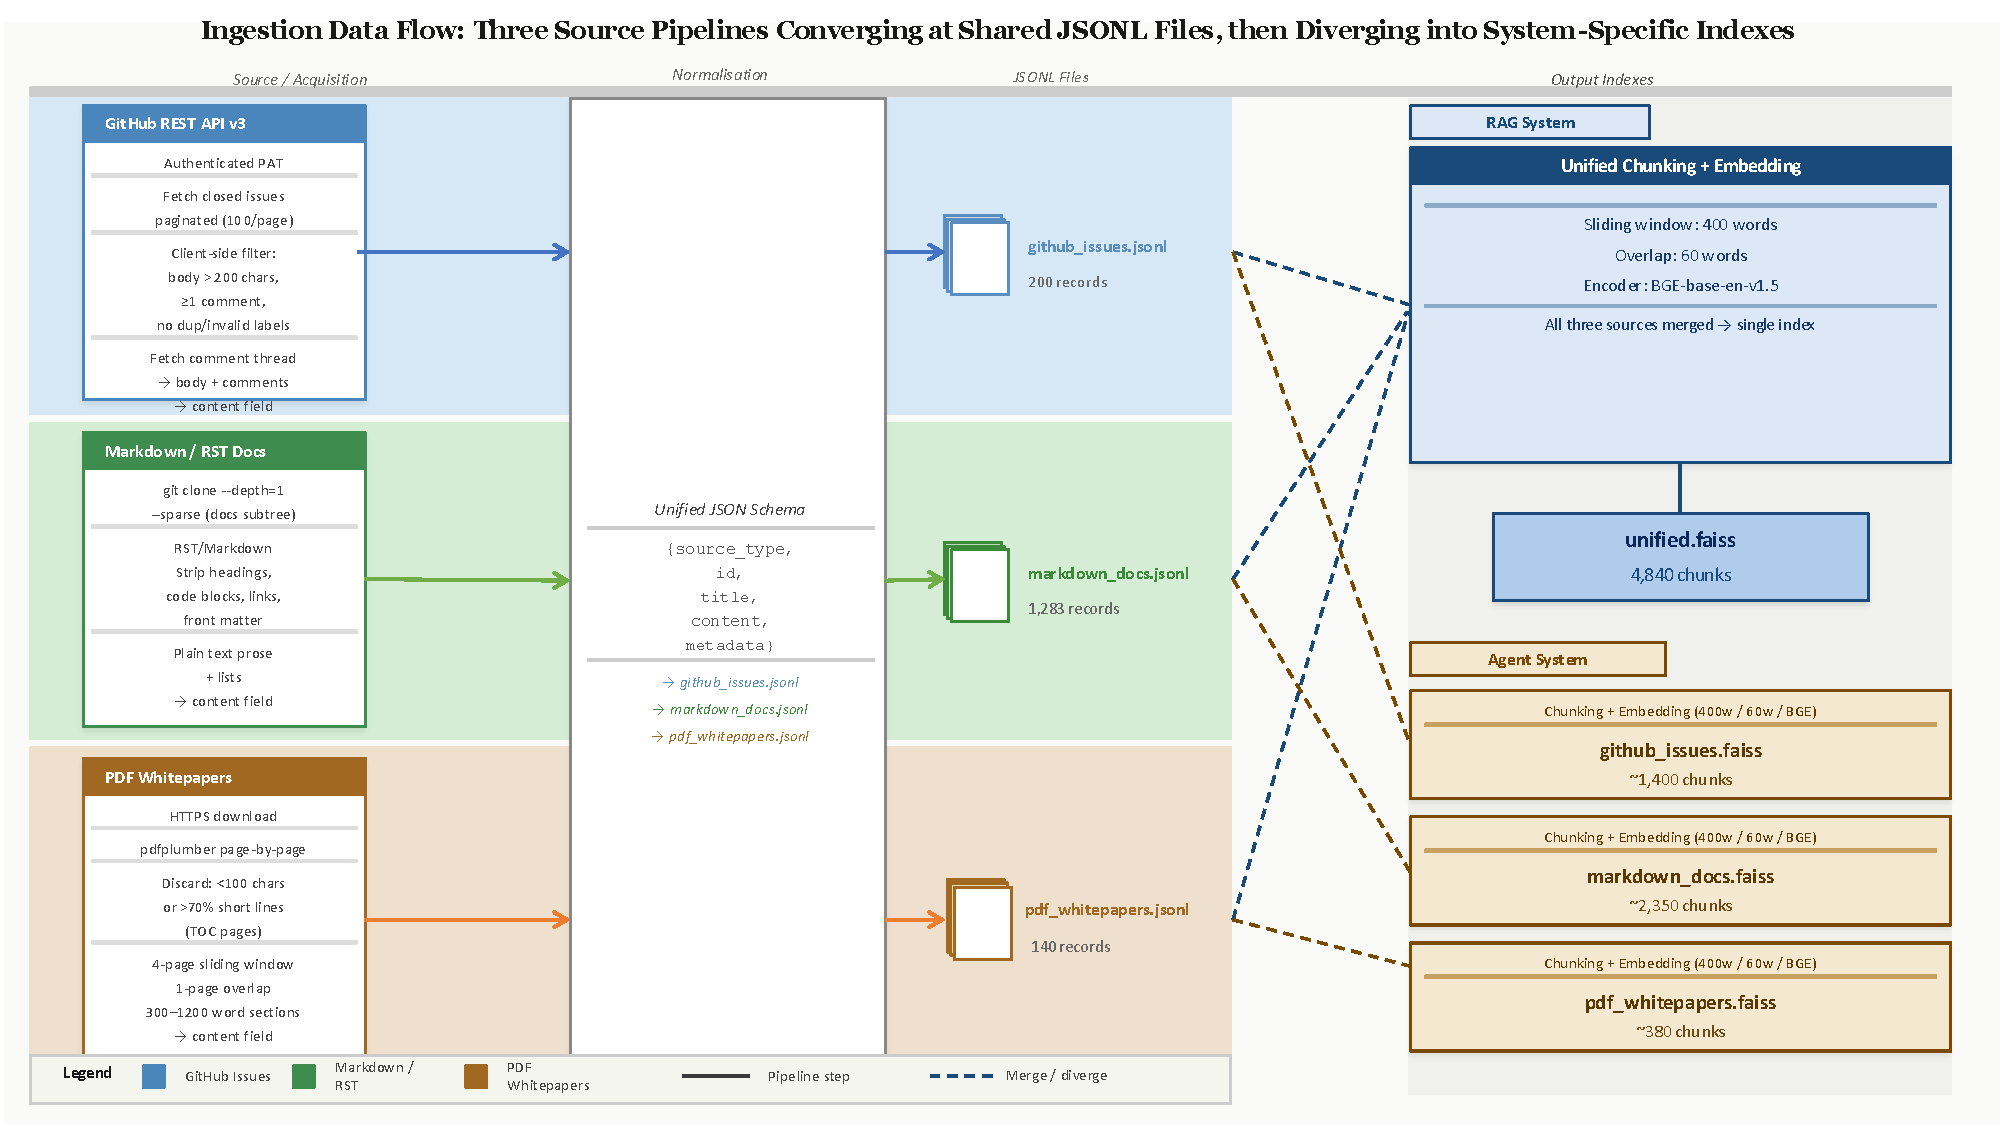
\includegraphics[width=\linewidth]{images/ingestion_flow}
  \caption{Ingestion data flow: three source pipelines converging at shared JSONL files, then diverging into system-specific indexes. Chunking parameters (400-word sliding window, 60-word overlap) and the BGE-base-en-v1.5 embedding model are shared across both systems; the sole architectural difference is a single unified index for RAG versus three per-source indexes for the agent.}
  \label{fig:dataflow}
\end{figure}

\textbf{GitHub Issues.} The GitHub REST API v3 is queried with an authenticated Personal Access Token, raising the rate limit from 60 to 5\,000 requests per hour. Closed issues are fetched in pages of 100, filtered client-side against the criteria defined in Section~\ref{ch:data}, and their comment threads are fetched in a subsequent request per issue. The body and comments are concatenated with a separator and written as a single \texttt{content} field.

\textbf{Markdown and RST documentation.} Repositories are cloned with \texttt{git clone \texttt{-{}-}depth=1 \texttt{-{}-}filter=blob:none \texttt{-{}-}sparse}, populating only the documentation subtree. This minimises bandwidth and avoids downloading build artefacts, themes, and binary assets. RST files from the Ansible documentation are processed identically to Markdown files; both formats are reduced to plain text by a regular-expression pipeline that strips headings, fenced code blocks, hyperlinks, shortcodes, and front matter, preserving only the readable prose and list content.

\textbf{PDF whitepapers.} PDFs are downloaded via authenticated HTTPS and processed with \texttt{pdfplumber}. Text is extracted page by page; pages with fewer than 100 characters of extracted text or exhibiting a table-of-contents structure (more than 70\,\% of lines shorter than 50 characters) are discarded. The remaining pages are grouped into overlapping four-page windows with a one-page overlap, producing sections of 300–1\,200 words that are large enough to contain coherent argumentation yet small enough to fit within a typical retrieval context window.

At the convergence point, both retrieval systems read from the same three JSONL files. The RAG pipeline passes all records through a single unified chunking and embedding stage, producing one vector index. The agent-based system ingests each JSONL file into a separate source-specific index, one per tool. This architectural divergence is one of the key design differences examined in the evaluation.

\section{Classical RAG Pipeline Architecture}

The classical RAG pipeline transforms raw corpus documents into a queryable knowledge store and, at query time, retrieves and synthesises the most relevant passages into a grounded answer. The implementation comprises eight discrete steps organised into two phases: an offline ingestion phase that runs once against the full corpus, and an online query phase that executes on every user request.

\subsection{Pipeline Stages}

Ingestion proceeds sequentially through four steps. Documents are loaded from the three source JSONL files, split into overlapping fixed-size chunks, encoded into dense vector representations by the embedding model, and added to a persistent FAISS index. At the end of ingestion, 1,623 corpus records have been expanded into 4,840 chunks, each carrying its parent document's source type, title, and metadata. The FAISS index and the chunk metadata store are written to disk and reloaded on startup, so the computationally intensive embedding step is never repeated unless the corpus changes.

The online query phase executes four further steps for each incoming question. The query is encoded by the same embedding model and the resulting vector is compared against all indexed chunk vectors to retrieve the twenty closest candidates. A cross-encoder reranker then scores each candidate against the query and returns the five highest-scoring chunks. These chunks are assembled into a numbered context block and passed to the language model alongside a system prompt that instructs the model to answer using only the supplied passages. Latency and token counts are captured for every query and appended to a structured JSONL log, producing the measurement records used in Chapter~\ref{ch:results}.

\subsection{Chunking Strategy}

Each corpus document is split into overlapping windows of 400 words with a 60-word overlap between consecutive windows. The step size between window starts is therefore 340 words, meaning that the first 60 words of each chunk also appear at the end of the preceding chunk. This overlap preserves semantic continuity across boundaries: a sentence or argument that spans a chunk boundary is fully represented in at least one chunk, ensuring that a relevant passage is not fragmented out of the index \cite{gao2023ragsurvey}.

Chunking operates on whitespace-delimited word lists rather than on subword tokens produced by a transformer tokeniser. This makes the chunking step independent of any specific model vocabulary, so that the embedding or reranker model can be replaced without recalibrating chunk sizes. In practice, a 400-word chunk corresponds to approximately 480–550 subword tokens for English technical prose, which falls within the 512-token context limit of the embedding model and well below the 8,192-token limit of the cross-encoder.

The 400-word target balances retrieval precision against contextual coherence, a trade-off documented explicitly in the Advanced RAG literature \cite{gao2023ragsurvey}. Shorter chunks increase the likelihood that a retrieved passage is topically homogeneous, but risk fragmenting multi-step arguments that require surrounding context to be interpretable; longer chunks preserve coherence but dilute the relevance signal. The 60-word overlap and 400-word window together place this implementation within the Advanced RAG category of the Naive / Advanced / Modular taxonomy, distinguishing it from Naive RAG pipelines that apply fixed splits without overlap.

\subsection{Embedding Model and Vector Store}

Chunks and queries are encoded using \texttt{BAAI/bge-base-en-v1.5}, a 768-dimensional bi-encoder model executed locally via the \texttt{sentence-transformers} library. The model was selected from the MTEB Retrieval leaderboard as a top-performing open-weight model at its parameter scale, requiring no external API call and incurring no per-token cost. BGE models are trained with an asymmetric query--document encoding scheme: at query time, the string \textit{``Represent this sentence for searching relevant passages:''} is prepended to the raw query before encoding, while document chunks are encoded without any prefix. This asymmetry is required for the model to produce embeddings that align query intent with document content; omitting the prefix at query time measurably degrades retrieval quality \cite{gao2023ragsurvey}.

All embeddings are L2-normalised to unit length before any similarity computation, both at ingestion time and at query time. Normalisation allows the FAISS \texttt{IndexFlatIP} index to compute cosine similarity via the inner product: for unit-length vectors $\mathbf{u}$ and $\mathbf{v}$, the relation $\mathbf{u} \cdot \mathbf{v} = \cos\theta$ holds, making inner-product maximisation equivalent to cosine similarity maximisation. Cosine similarity is preferred over raw inner product because it is magnitude-invariant — a longer chunk does not receive a spuriously high score simply by virtue of producing a larger embedding vector.

FAISS \texttt{IndexFlatIP} performs exact nearest-neighbour search over the full index without quantisation or approximation. At 4,840 vectors of dimension 768 stored as 32-bit floats, the index occupies approximately 14\,MB of memory and returns query results in under one second on the development hardware. Exact search is therefore practical at this corpus scale and avoids the recall penalty introduced by approximate methods such as HNSW or IVF clustering, which trade retrieval accuracy for speed at larger scales \cite{lewis2020rag}.

\subsection{Retrieval and Reranking}

Retrieval proceeds in two stages to exploit the complementary properties of bi-encoders and cross-encoders. In the first stage, the FAISS index returns the twenty document chunks whose embeddings have the highest cosine similarity to the embedded query. These twenty candidates are then passed to \texttt{cross-encoder/ms-marco-MiniLM-L-6-v2}, a cross-encoder model fine-tuned on the MS MARCO passage-ranking benchmark, which scores each query--chunk pair jointly by processing the concatenated pair as a single transformer input.

The key distinction between the two stages lies in how query and document representations are produced. Bi-encoders encode queries and documents independently and compare them post hoc; this enables sub-second retrieval over arbitrarily large indexes but prevents the model from attending to fine-grained token-level interactions between the two texts. Cross-encoders process both texts as a single input, allowing full cross-attention across the query--chunk boundary and producing substantially more accurate relevance scores at the cost of one forward pass per candidate \cite{gao2023ragsurvey}. Applying the cross-encoder only to the twenty FAISS candidates bounds its computational cost to a fixed and small number of inference calls regardless of index size, keeping online latency predictable.

The five highest-scoring chunks after reranking are passed to the generator. Each chunk carries both its FAISS cosine similarity score and its cross-encoder rerank score in the log record, providing a complete provenance trail for post-hoc analysis of retrieval behaviour. Temperature is set to zero for all generation calls to ensure fully deterministic outputs across evaluation runs, a requirement for the reproducibility of the evaluation described in Chapter~\ref{ch:data}. Two retrieval enhancements extend this baseline. Both were incorporated as a post-evaluation revision to the pipeline; the initial results that motivated their addition are presented in Chapter~\ref{ch:results}, and their implementation is detailed in Section~\ref{sec:rag-impl}.

\textbf{Hypothetical Document Embedding (HyDE)} addresses the semantic mismatch between query register and document register that constrains bi-encoder retrieval \cite{gao2023hyde}. Before querying the FAISS index, the language model generates a short hypothetical passage — two to three sentences — that directly answers the query. This passage is embedded without the BGE retrieval prefix, placing its vector in the same distributional region as stored document chunks rather than in the query subspace. The hypothesis vector replaces the query vector as the FAISS search input; the original query is preserved and used unchanged for cross-encoder reranking, so relevance scoring remains grounded in the actual question rather than in the generated passage.

\textbf{Maximal Marginal Relevance (MMR)} addresses the tendency of nearest-neighbour retrieval to return near-duplicate passages from the same document section \cite{carbonell1998mmr}. After the cross-encoder sorts the twenty candidates by relevance, MMR iteratively selects the five final passages by maximising a linear combination of relevance and diversity: at each step it picks the candidate that best balances a high normalised rerank score against low cosine similarity to the passages already selected. A relevance weight of $\lambda = 0.7$ gives relevance priority over diversity, ensuring the final context window is both topically focused and non-redundant. Figure~\ref{fig:rag_pipeline} illustrates the complete query-phase pipeline including both extensions.

\begin{figure}[ht]
  \centering
  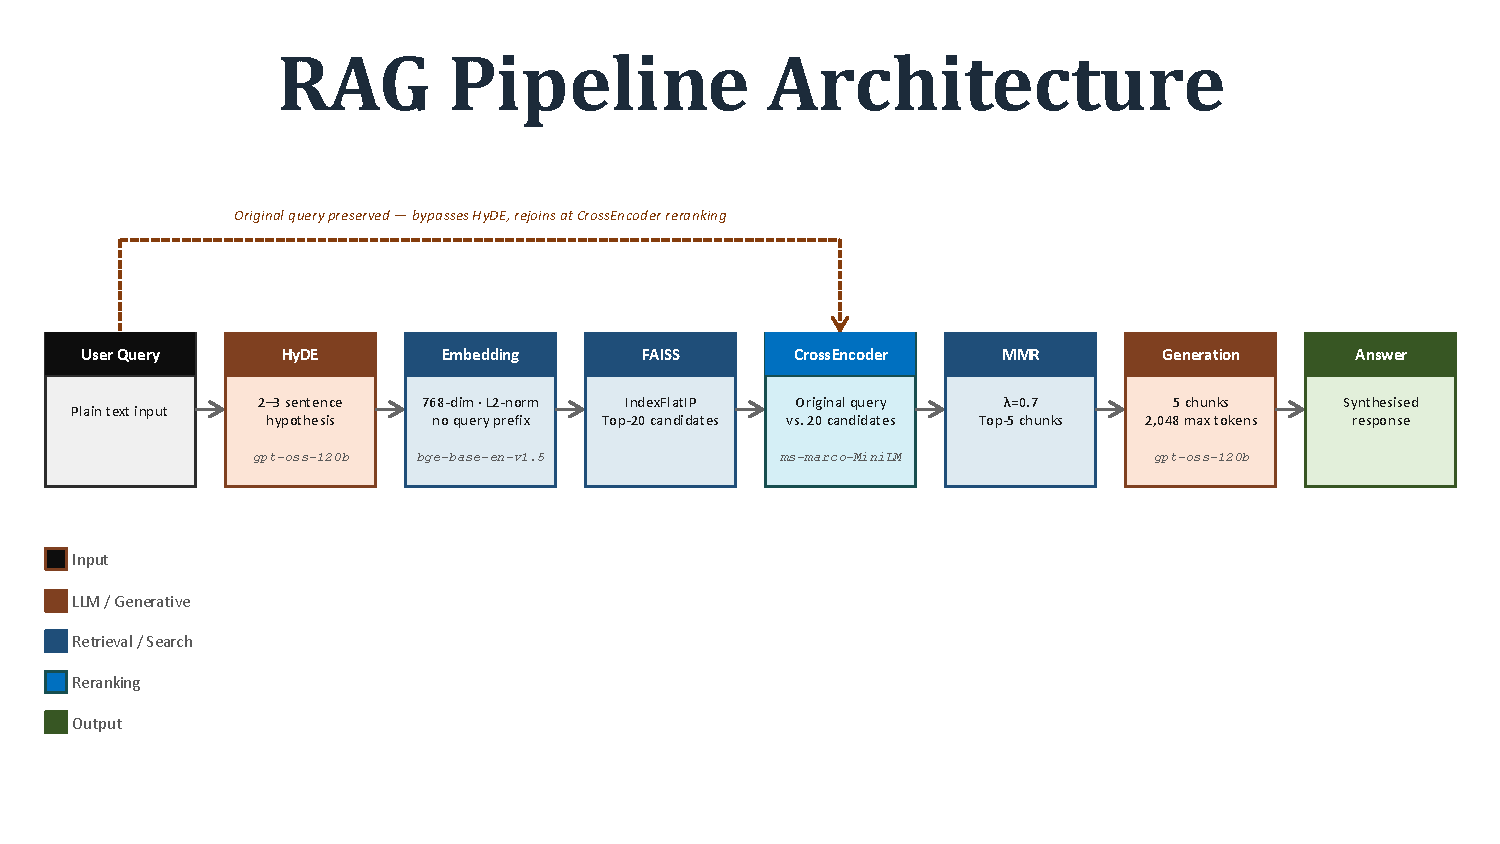
\includegraphics[width=\linewidth]{images/rag_pipeline}
  \caption{RAG pipeline query phase. The original query is passed to the LLM to generate a hypothetical passage (HyDE), whose embedding is used as the FAISS search vector. The original query is preserved for cross-encoder reranking, ensuring relevance scoring remains grounded in the actual question. MMR diversification ($\lambda = 0.7$) then selects the final five passages from the reranked pool before synthesis.}
  \label{fig:rag_pipeline}
\end{figure}

\section{Agent-Based System Architecture}

The agent-based system replaces the RAG pipeline's fixed retrieve-then-generate sequence with an iterative reasoning loop in which the language model selects and invokes retrieval tools based on the content and requirements of each query. Rather than encoding the entire corpus into a single unified index, the system exposes three source-specific retrieval tools and delegates the decision of which tool to call, in what order, and with what query formulation to the language model at runtime. The implementation follows the ReAct framework \cite{yao2023react} and is built using LangChain's agent scaffolding on top of the same language model endpoint and embedding infrastructure used by the RAG pipeline.

\subsection{The Agent Loop}

ReAct defines an interleaved reasoning and acting pattern in which a language model alternates between generating a \textit{Thought}—an explicit natural-language reasoning step—and taking an \textit{Action}—a structured tool call with explicit inputs \cite{yao2023react}. After each action, the tool's return value is appended to the context as an \textit{Observation}, and the model continues reasoning from the updated context until it emits a final answer prefixed with the token \textit{Final Answer}. This cycle constitutes a closed-loop process: unlike the single retrieval pass of the RAG pipeline, the agent can inspect retrieved evidence, judge its sufficiency, and issue further tool calls or reformulated queries before committing to a response.

The implementation uses LangChain's \texttt{create\_react\_agent} function, which binds the language model, the registered tool set, and a ReAct-format prompt into an executable agent definition, and \texttt{AgentExecutor}, which drives the reasoning cycle at runtime. The language model is accessed through LangChain's \texttt{ChatOpenAI} wrapper pointed at the same OpenAI-compatible endpoint used by the RAG pipeline—Ollama in development, AI Refinery during evaluation—with identical model identifier and temperature settings. A maximum iteration count of fifteen is enforced by the \texttt{AgentExecutor}; this bound accommodates queries that require all three tools in sequence while preventing unbounded loop growth on ambiguous or unanswerable inputs.

\subsection{Tools and Source Routing}

Three retrieval tools are registered with the agent, one per corpus source type. Each tool wraps a dedicated FAISS index constructed from the same corpus using the same 400-word sliding-window chunking, 60-word overlap, and BGE-base-en-v1.5 embedding model as the RAG pipeline. Separate per-source indexes are used rather than the RAG pipeline's unified index to reflect the architectural reality of enterprise knowledge environments, in which issue trackers, documentation platforms, and document repositories are independent systems with distinct search interfaces \cite{ferrazzi2026agenticrag}. An agent operating over a unified index would have no structural basis on which to make source-routing decisions; partitioning the indexes makes routing a genuine runtime choice with observable consequences for retrieval quality and, consequently, answer faithfulness.

\begin{table}[ht]
\centering
\small
\setlength{\tabcolsep}{4pt}
\caption{Agent retrieval tools and their source-type scope.}
\label{tab:agent_tools}
\begin{tabular}{lll}
\hline
\textbf{Tool name} & \textbf{Source type} & \textbf{Enterprise proxy} \\
\hline
\texttt{search\_github\_issues}   & GitHub Issues     & Jira tickets \\
\texttt{search\_markdown\_docs}   & Markdown/RST docs & Confluence wiki \\
\texttt{search\_pdf\_whitepapers} & CNCF PDF sections & SharePoint documents \\
\hline
\end{tabular}
\end{table}

Each tool applies the same two-stage retrieval used in the RAG pipeline: twenty nearest-neighbour candidates are retrieved from the tool's FAISS index and then reranked by \texttt{cross-encoder/ms-marco-MiniLM-L-6-v2} to a top-five result set. This ensures that retrieval quality per tool call is directly comparable to the RAG pipeline's retrieval quality, so that any differences in final answer quality reflect the agent's routing and synthesis behaviour rather than differences in the underlying retrieval mechanics.

\subsection{Orchestration Logic}

Source routing is implemented entirely through the natural-language descriptions attached to each tool in the ReAct system prompt. No explicit rule-based dispatch logic is implemented; the language model reads each tool's description and selects the appropriate tool based on query semantics at each reasoning step. The descriptions are written to reflect the structural characteristics and dominant query patterns of each source type: the GitHub Issues tool is described as appropriate for bug reports, error messages, and issue resolutions; the documentation tool for conceptual explanations, how-to guides, and configuration references; the whitepaper tool for standards, best practice recommendations, and maturity frameworks. This design is authentic to the ReAct pattern, in which tool selection is part of the Thought generation step \cite{yao2023react}, and avoids brittle keyword-based dispatch that would require maintenance whenever the corpus is extended.

Tool observations are returned as formatted plain text containing the five reranked chunks, each prefixed with its source type, document title, and cosine similarity score. This format supplies the language model with the provenance information required to attribute claims and to judge whether a further tool call is warranted, while keeping each observation compact enough to avoid exhausting the context window across multi-step queries. The agent may call the same tool more than once with a reformulated query if the first observation is insufficient, or it may call multiple tools in sequence for cross-source synthesis queries.

All tool calls, their inputs, and their observations are recorded in a structured \texttt{agent\_trace} field appended to each log record alongside the query, final answer, total latency, and token counts. The log schema is a strict superset of the RAG pipeline's schema: all shared fields—query, answer, latency, token counts, and retrieved chunks—are produced identically by both systems, while the \texttt{agent\_trace}, tool-call count, and source-routing fields are present only in agent logs. This shared outer schema ensures that the evaluation infrastructure processes both systems' outputs without modification. Figure~\ref{fig:single_agent} illustrates the complete single-agent loop.

\begin{figure}[ht]
  \centering
  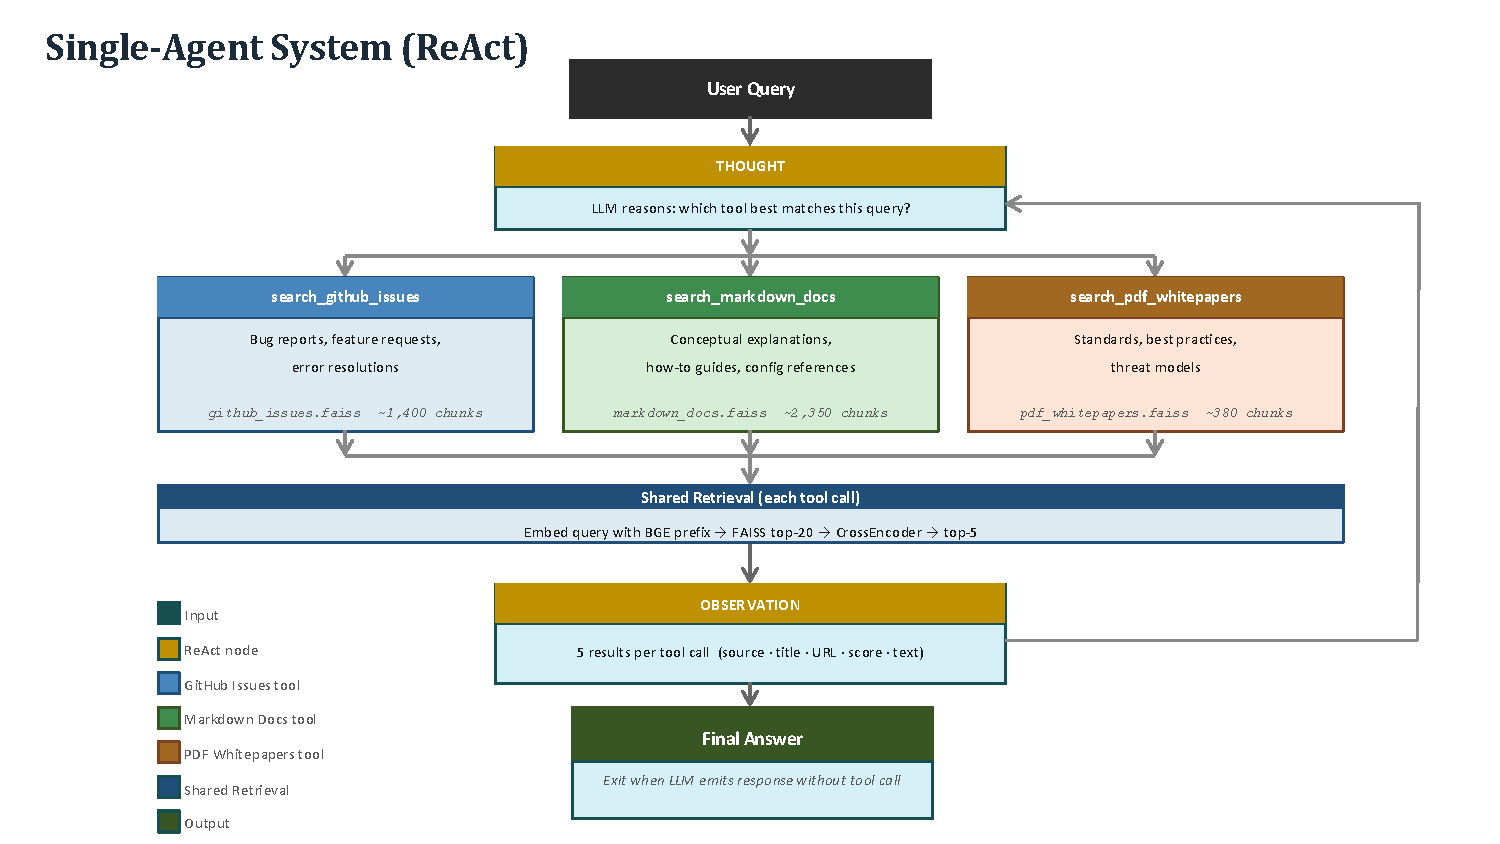
\includegraphics[width=\linewidth]{images/single_agent}
  \caption{Single-agent ReAct loop. The language model alternates between Thought (reasoning) and Action (tool call) steps; each tool observation is appended to the growing context window and the cycle repeats until the model emits a final answer without a tool call, or the 15-iteration ceiling is reached.}
  \label{fig:single_agent}
\end{figure}

\subsection{Multi-Agent Coordination Architecture}
\label{subsec:multi-agent-design}

The multi-agent architecture was designed as a corrective response to structural failure modes identified during single-agent evaluation: context accumulation across the ReAct loop exhausted the iteration ceiling, causing 41~per cent of queries to fail before a final answer was produced. Rather than lengthening the iteration limit further, the architecture eliminates the loop entirely.

\begin{sloppypar}
The design is a two-node LangGraph \texttt{StateGraph}. The first node, \texttt{retrieve\_all\_sources}, queries all three source-specific FAISS indexes sequentially — GitHub Issues, Markdown documentation, and PDF whitepapers — applying the same cross-encoder reranking pipeline used in both the RAG and single-agent systems to each source in turn, and accumulating at most fifteen chunks in total, five per source. The second node, \texttt{synthesize}, receives the pooled passages as a single bounded context window and issues exactly one language model call to produce the final answer. No further retrieval is possible once synthesis begins; the context presented to the model is fixed at the point the first node completes.
\end{sloppypar}

Three design properties distinguish this architecture from the single-agent system. There is no reasoning loop and therefore no iteration limit and no risk of\linebreak[0] \texttt{GraphRecursionError}. The context window per query is fixed at fifteen chunks regardless of query type or complexity, making the per-query token budget fully predictable. All three sources are queried on every request, so source coverage is an architectural guarantee rather than a model-driven decision \cite{xi2023rise}. These properties come at a cost: the multi-agent system cannot direct retrieval effort selectively toward the most relevant source, nor can it reformulate a query after inspecting an initial observation.

The multi-agent reuses the per-source FAISS indexes constructed by \texttt{agent/ingest.py} and the \texttt{SourceRetriever} class from \texttt{agent/tools.py}, adding no new ingestion infrastructure. The primary trade-off relative to the single agent is coverage guarantee versus query-adaptive selectivity: the multi-agent provides complete source coverage at the cost of the ability to concentrate retrieval on a single source for queries whose answer is localised to one part of the corpus. Figure~\ref{fig:multi_agent} illustrates the architecture.

\begin{figure}[ht]
  \centering
  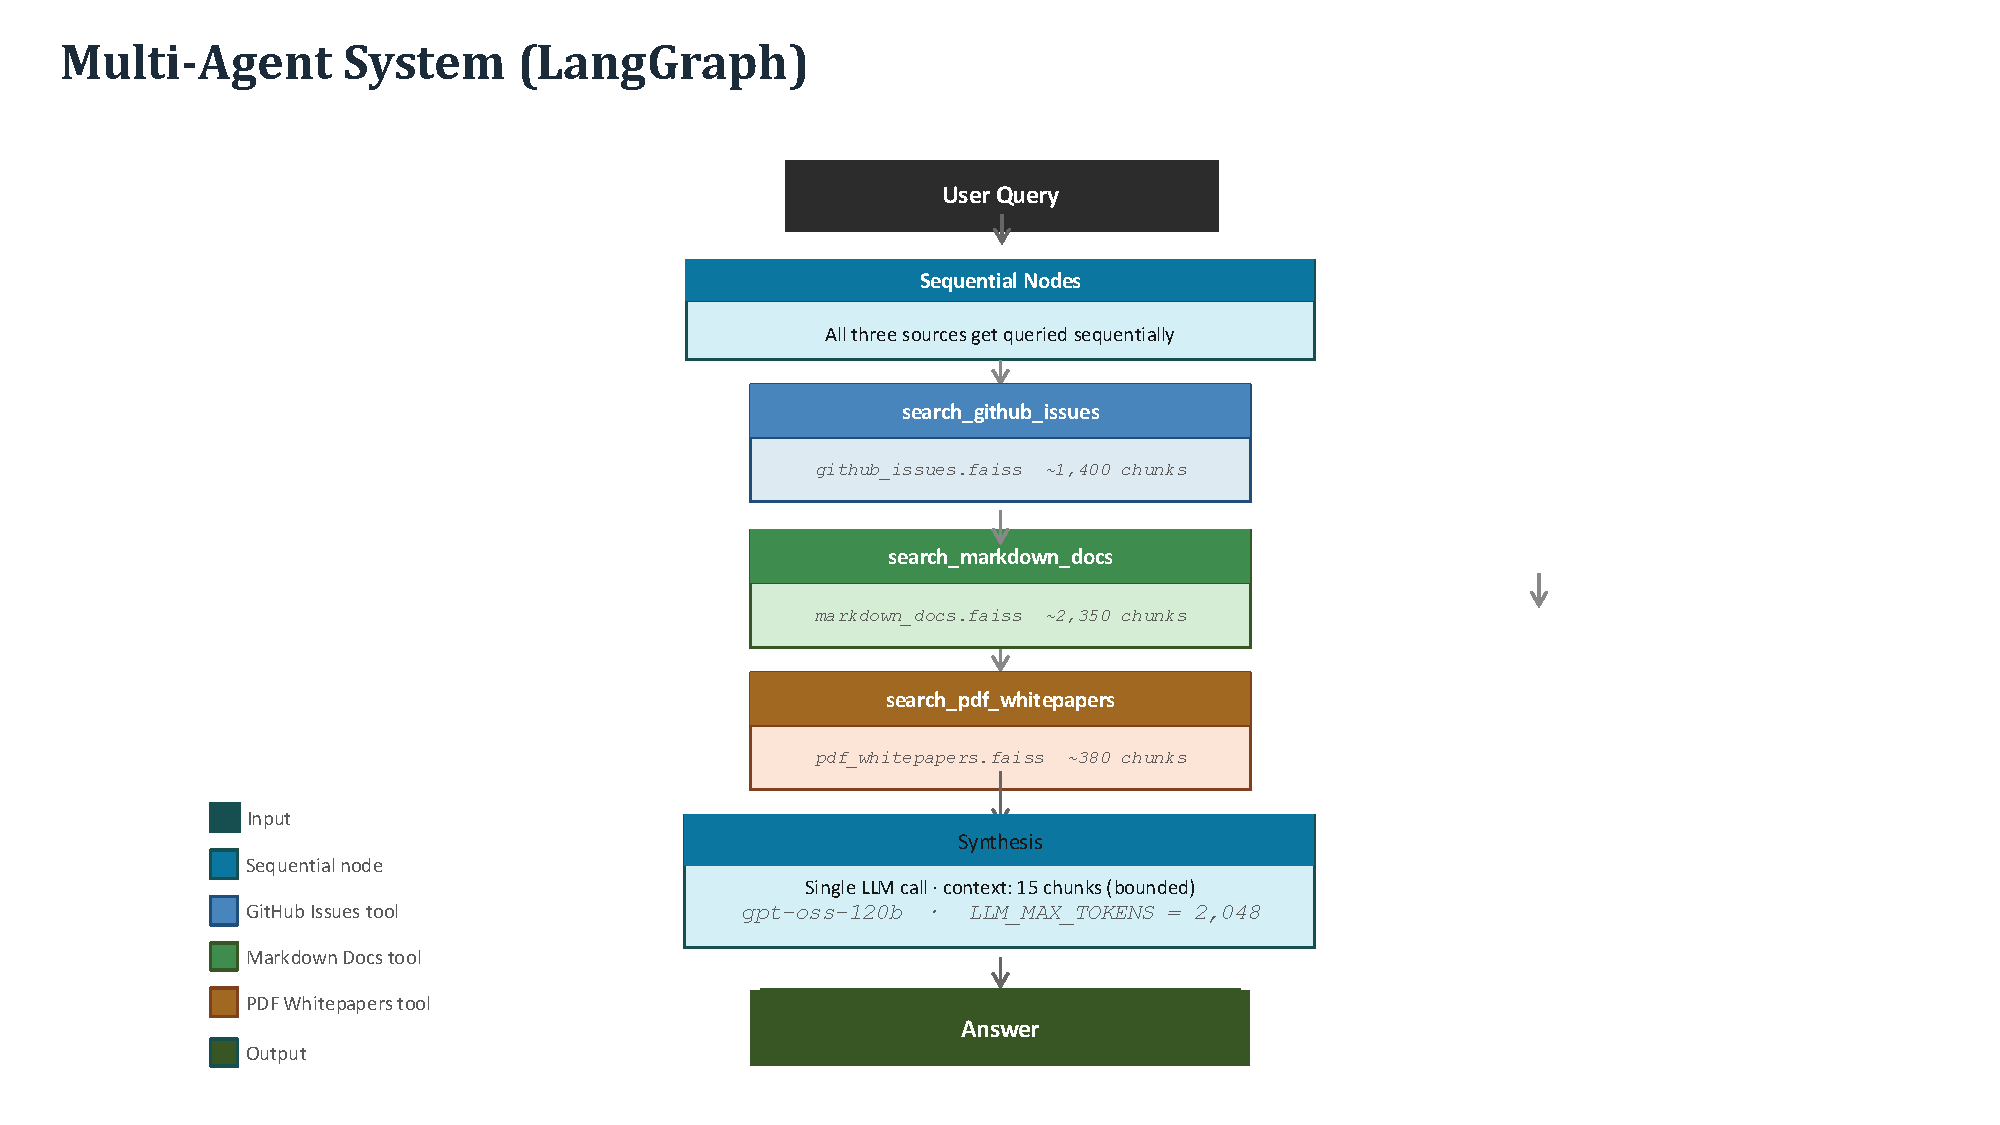
\includegraphics[width=\linewidth]{images/multi_agent}
  \caption{Multi-agent coordination architecture. A single \texttt{retrieve\_all\_sources} node queries all three per-source FAISS indexes sequentially, accumulating five chunks per source. The \texttt{synthesize} node then issues exactly one LLM call over the pooled fifteen-chunk context. There is no reasoning loop and no iteration limit.}
  \label{fig:multi_agent}
\end{figure}

\section{Comparability Design Decisions}

A valid architectural comparison requires that observed differences in evaluation outcomes be attributable to the retrieval and orchestration strategies under study rather than to differences in data, models, or hardware. Every component not itself under comparison is therefore held constant across both systems. Table~\ref{tab:comparability} lists the shared and varied parameters; the design decisions implicit in each row are elaborated below.

\subsection{Shared Experimental Parameters}

The language model, embedding model, chunking parameters, and reranker are identical across both systems. Both access the language model through the same OpenAI-compatible endpoint—Ollama locally, AI Refinery for evaluation—using the same model identifier and a generation temperature of zero. Temperature is fixed at zero to produce fully deterministic outputs; any repeated query to either system yields the same response, which is a prerequisite for reliable latency averaging and reproducible RAGAS scoring. Both systems embed queries and corpus chunks using \texttt{BAAI/bge-base-en-v1.5} with L2-normalised vectors and the same retrieval-prefix convention, and both apply \texttt{cross-encoder/ms-marco-MiniLM-L-6-v2} to a candidate pool of twenty, returning five chunks as the final retrieved context.

\begin{table}[ht]
\centering
\small
\setlength{\tabcolsep}{4pt}
\caption{Controlled and varied parameters across both systems.}
\label{tab:comparability}
\begin{tabular}{p{3.8cm}p{5.4cm}p{5.4cm}}
\hline
\textbf{Parameter} & \textbf{RAG Pipeline} & \textbf{Agent System} \\
\hline
Language model        & shared endpoint; swapped via \texttt{.env} & shared endpoint; swapped via \texttt{.env} \\
Embedding model       & BGE-base-en-v1.5 (768d)     & BGE-base-en-v1.5 (768d) \\
Chunking              & 400 words, 60-word overlap  & 400 words, 60-word overlap \\
Reranker              & MiniLM, top-5               & MiniLM, top-5 per tool call \\
Document corpus       & shared JSONL source files   & shared JSONL source files \\
Generation temperature & 0 (deterministic)          & 0 (deterministic) \\
Hardware and runtime  & local CPU, single venv      & local CPU, single venv \\
\hline
\textit{Index structure}  & Unified FAISS (4\,840 chunks) & Three per-source FAISS indexes \\
\textit{Query resolution} & Fixed 4-step pipeline         & Iterative loop, max 15 steps \\
\textit{Source routing}   & Implicit (unified index)      & Explicit (LLM tool selection) \\
\hline
\end{tabular}
\end{table}

The document corpus is shared at the source level: both systems read from the same three JSONL files in \texttt{data/corpus/}. Their index structures differ because the RAG pipeline consolidates all records into a single FAISS index while the agent builds three separate per-source indexes from the same files. The total chunk count differs marginally—4,840 in the unified index versus approximately 4,130 across the three agent indexes—because the Markdown corpus is lightly downsampled during agent ingestion to keep index sizes balanced. Both systems run in the same Python virtual environment on the same hardware, eliminating interpreter version, library dependency, and process-level differences as confounds in the latency measurements.

\subsection{Defining Equivalent Effort}

Implementation complexity is evaluated as a first-class metric in this thesis, corresponding to Research Question 3. To make this comparison defensible, complexity is operationalised through three observable proxies rather than through subjective judgements about code quality or design elegance.

Lines of non-blank, non-comment code are counted per component for four parallel components in each system: ingestion, retrieval or tools, generation or agent executor, and the pipeline orchestrator. Framework calls—including LangChain agent and tool definitions—count toward the agent's total, because they represent integration and configuration work a developer must write and maintain. The second proxy is the number of explicit configuration parameters in each system's \texttt{config.py} file, reflecting the number of decisions a practitioner must make to deploy or tune the system. The third proxy is the number of steps required to onboard a new data source: for the RAG pipeline this involves appending records to the unified ingestion script and re-running the embedding step; for the agent it additionally requires building a new per-source FAISS index, writing a new \texttt{@tool} function, and updating the tool descriptions in the system prompt. These three proxies together provide an objective basis for the rubric-based complexity scores presented in Chapter~\ref{ch:results}.

	%!TEX root = ../dokumentation.tex

\chapter{Data and Evaluation Setup}
\label{ch:data}

\section{Dataset Construction}
\label{sec:dataset}

The corpus used in this evaluation was assembled from three structurally distinct open-source document collections, each selected as a proxy for a category of enterprise knowledge source. Collection, preprocessing, and normalisation were automated through three Python scripts — \texttt{01\_fetch\_github\_issues.py}, \texttt{02\_fetch\_markdown\_docs.py}, and \texttt{03\_fetch\_pdfs.py} — executed against publicly accessible repositories and APIs. All records were written to the unified JSONL schema defined in Section~\ref{ch:design} before being consumed by either retrieval system.

\subsection{Data Collection per Source Type}

\textbf{GitHub Issues.} Issues were retrieved from \texttt{kubernetes/kubernetes} and \texttt{microsoft/vscode} via the GitHub REST API v3 using a Personal Access Token, which raises the authenticated rate limit from 60 to 5\,000 requests per hour. A target of 100 qualifying issues per repository was set, yielding a maximum corpus of 200 records. Four filter criteria were applied during collection: only closed issues were fetched, because closed records contain resolution context alongside the original problem description; the issue body was required to exceed 200 characters, excluding stub entries; at least one comment was required, ensuring discussion beyond the opening post; and issues carrying the labels \textit{duplicate}, \textit{invalid}, or \textit{wontfix} were discarded. Pull requests, which share the GitHub issues endpoint, were identified and excluded via the presence of a \texttt{pull\_request} field in the API response. For each qualifying issue, a separate request retrieved up to 50 comments; the issue body and all comment texts were concatenated with a separator into a single \texttt{content} field.

\textbf{Markdown and RST documentation.} Three repositories were cloned using \texttt{git clone \texttt{-{}-}depth=1 \texttt{-{}-}filter=blob:none \texttt{-{}-}sparse} to minimise bandwidth by downloading only the relevant documentation subtree. From \texttt{kubernetes/website}, only the \texttt{content/en/docs} directory was checked out, yielding Markdown files from the official Kubernetes documentation. From \texttt{ansible/ansible-documentation}, the \texttt{docs/} directory was checked out, containing both Markdown and RST files. The \texttt{cncf/tag-observability} repository was cloned in full, as it is a small repository whose content — including the 68\,KB observability whitepaper and working-group documents — is distributed across the root and subdirectories. Directories that contain navigation scaffolding, theme assets, and non-prose content were excluded by path matching against a fixed skip-list (\texttt{assets}, \texttt{static}, \texttt{themes}, \texttt{\_layouts}, and equivalents). Files smaller than 1\,KB were discarded before markup stripping.

\textbf{PDF whitepapers.} Fourteen CNCF documents were downloaded via HTTPS from five repositories: \texttt{cncf/tag-security} (five documents, \texttt{main} branch), \texttt{cncf/tag-storage} (two documents, \texttt{master} branch), \texttt{cncf/tag-app-delivery} (three documents), \texttt{cncf/foundation} (two documents), and \texttt{cncf/wg-serverless} (one document, \texttt{master} branch). Text was extracted page by page using \texttt{pdfplumber}. Pages were classified as junk and discarded if they contained fewer than 100 characters of extracted text or if more than 70\,\% of their non-empty lines were shorter than 50 characters — a heuristic that reliably identifies cover pages and table-of-contents pages without requiring heading detection. The CNCF AI-assisted development survey yielded zero extractable text pages due to a graphics-only layout and was excluded from the corpus. The remaining 13 documents were segmented into overlapping four-page windows with a one-page overlap, producing sections of coherent prose suitable for retrieval.

\subsection{Preprocessing and Normalisation}

Markdown and RST files were reduced to plain text by a regular-expression pipeline that removed YAML front matter, fenced code blocks, inline code spans, HTML tags, Hugo shortcodes, and Markdown image references. Markdown hyperlinks were reduced to their display label; RST roles were similarly reduced to their content. RST structural underline characters and directive declarations were removed. Consecutive blank lines were collapsed to a single blank line. This pipeline was applied uniformly to both Markdown and RST files; no format-specific branch was required beyond the removal of RST-specific syntax. All records from the documentation and PDF sources were capped at 8\,000 characters after stripping, preventing any single document from dominating retrieval contexts. GitHub issue content was not capped at this stage, as issue bodies and comment threads are segmented into 400-word overlapping chunks during index construction.

Every record produced by each acquisition script was written to the same five-field JSONL schema — \texttt{source\_type}, \texttt{id}, \texttt{title}, \texttt{content}, \texttt{metadata} — described in Section~\ref{ch:design}. No cross-source deduplication was performed, as the three source types draw from non-overlapping repositories with non-overlapping document namespaces. Within each source, uniqueness is guaranteed by the issue number (GitHub), the file path relative to the repository root (Markdown), and the document name plus section index (PDF).

\subsection{Corpus Statistics}

The completed corpus contains 1\,623 records across the three source types, with a combined total of approximately 1\,449\,000 words. Table~\ref{tab:corpus_stats} reports per-source record counts, word-length statistics, and estimated token counts; the token estimates assume an average of 1.3 subword tokens per English word, consistent with the BGE tokeniser's subword vocabulary for technical prose.

\begin{table}[ht]
\centering
\small
\setlength{\tabcolsep}{4pt}
\caption{Corpus statistics after acquisition, filtering, and normalisation.}
\label{tab:corpus_stats}
\begin{tabular}{lrrrr}
\hline
\textbf{Source type} & \textbf{Records} & \textbf{Avg words} & \textbf{Total words} & \textbf{Approx.\ tokens} \\
\hline
GitHub Issues        & 200   & 2\,434 & 486\,826   & 633\,000 \\
Markdown / RST docs  & 1\,283 & 646   & 829\,088   & 1\,078\,000 \\
PDF whitepaper sections & 140 & 952   & 133\,281   & 173\,000 \\
\hline
\textbf{Total}       & \textbf{1\,623} & & \textbf{1\,449\,195} & \textbf{1\,884\,000} \\
\hline
\end{tabular}
\end{table}

GitHub issues show the widest length variation: the distribution spans from brief issue stubs that passed the 200-character body filter to multi-comment threads exceeding 2\,000 words, with the majority falling between 200 and 500 words after the body and comments are concatenated. Markdown documents are tightly bounded by the 8\,000-character content cap, producing a maximum of approximately 1\,400 words per record and a distribution concentrated between 500 and 1\,000 words. PDF sections, also capped at 8\,000 characters, are the most length-uniform source: 88 of 140 sections fall in the 1\,000--2\,000-word range, reflecting the dense prose typical of formal technical whitepapers. The length diversity across source types mirrors the structural heterogeneity of the enterprise environment this corpus is designed to simulate.

\section{Evaluation Query Set}

\subsection{Synthetic QA Generation}

Candidate question--answer pairs are generated by prompting \texttt{gpt-oss-120b}, accessed through the Accenture AI Refinery endpoint, against corpus excerpts sampled from the indexes built in Section~\ref{sec:dataset}. This LLM-assisted approach is established practice for constructing domain-specific evaluation benchmarks when no annotated dataset exists \cite{es2023ragas}. Using the same model for generation and for answer evaluation, rather than a separate weaker generator, keeps phrasing conventions consistent between ground-truth answers and the system outputs under evaluation, which reduces spurious penalties in semantic similarity scoring.

One structured prompt template was designed for each query type; all templates instruct the model to return a JSON object containing the question, the ground-truth answer, and the list of source chunk identifiers forming the evidence base. The prompt for factual and synthesis questions specifies three requirements: the question must be answerable solely from the provided passage or passages, the wording must not quote or paraphrase the answer, and the question must be specific enough to admit exactly one correct answer. Responses are parsed with \texttt{json.loads}; responses that fail to parse or violate the expected schema are discarded before human review. The generation script, \texttt{scripts/evaluation/generate\_queries.py}, handles chunk sampling, prompt construction, API calls, and result storage. All generated candidates are written to \texttt{data/eval/candidates.jsonl}; the final reviewed set is stored in \texttt{data/eval/queries.jsonl} under the schema defined in Table~\ref{tab:query_schema}.

\subsection{Query Taxonomy}

The evaluation set contains 90 queries organised into four types, each designed to stress one of Gao et al.'s four RAG capability dimensions \cite{gao2023ragsurvey}. Table~\ref{tab:query_taxonomy} summarises the taxonomy. Structuring the query set around these dimensions makes the comparison between systems directly interpretable in terms of the literature: performance differences on each subset can be attributed to a specific aspect of retrieval behaviour rather than to undifferentiated query difficulty.

\begin{table}[ht]
\centering
\small
\setlength{\tabcolsep}{4pt}
\caption{Evaluation query taxonomy: four types mapping to Gao et al.'s RAG capability dimensions.}
\label{tab:query_taxonomy}
\begin{tabular}{p{2.4cm}p{4.0cm}rp{6.0cm}}
\hline
\textbf{Type} & \textbf{Capability dimension} & \textbf{Count} & \textbf{Description} \\
\hline
Factual      & Noise robustness         & 30 & Single-chunk answer; one source type \\
Synthesis    & Information integration  & 30 & Answer spans 2+ passages; $\geq$10 cross-source \\
Ambiguous    & Noise robustness         & 15 & Underspecified query; no unique correct answer \\
Unanswerable & Negative rejection       & 15 & Plausible but corpus-absent topic \\
\hline
\textbf{Total} &                        & \textbf{90} & \\
\hline
\end{tabular}
\end{table}

\textbf{Factual queries} each have a single correct answer contained within one corpus chunk. The generation script samples chunks stratified by source type---17 from Markdown documentation, 17 from GitHub issues, and 16 from PDF whitepapers---and prompts the model to produce one factual question per chunk. After manual review, the accepted set is balanced to approximately 10 questions per source type.

\textbf{Synthesis queries} require combining information from at least two passages to answer correctly. Chunk pairs were sampled in three configurations: pairs from within the same document, pairs from different documents of the same source type, and pairs spanning two distinct source types (cross-source). Approximately 12 of the 40 sampled pairs are cross-source; the review process requires that at least 10 cross-source questions survive to the final set. Cross-source synthesis queries are structurally important for the agent evaluation: they require the agent to invoke multiple tools rather than resolving the query from a single index, making routing accuracy directly observable.

\textbf{Ambiguous queries} are derived from accepted factual questions by removing one key identifying term---the technology name, the version specifier, or the system being described---and prompting the model to rewrite the result as a naturally underspecified query. The rewritten question remains plausible and domain-relevant but lacks the context required to return a unique correct answer. Approximately five ambiguous queries target each source type.

\textbf{Unanswerable queries} are composed by hand rather than generated by a language model, because a model prompted against corpus excerpts cannot reliably invent plausible questions about topics the corpus does not contain. Each unanswerable question concerns a topic adjacent to the corpus domain but absent from every source---for example, Kubernetes features introduced after the issue snapshot date, security standards not referenced in any whitepaper, or Ansible modules absent from the documentation clone. Each candidate is verified by running it through both retrieval systems and confirming that no top-5 retrieved chunk provides a sufficient answer.

\subsection{Manual Review and Filtering}

Every LLM-generated candidate undergoes manual review before acceptance into the final query set. A candidate is accepted if six criteria are satisfied: the ground-truth answer is directly verifiable against the cited source text without inference beyond what is written; the question wording does not quote or paraphrase the answer; the question is non-trivial in the sense that a keyword match on its surface terms is insufficient to locate the answer; for synthesis candidates, the answer cannot be produced from any single chunk in isolation and both cited passages are genuinely required; for ambiguous candidates, the rewritten question reads naturally and would plausibly be asked by a domain non-expert; and the English is clear, well-formed, and domain-appropriate. A candidate is rejected if its answer admits multiple valid interpretations, if the question is a near-verbatim copy of a sentence from the source text, or if a correct answer requires domain knowledge not present in the corpus.

Rejected candidates are deleted from \texttt{data/eval/candidates.jsonl}; accepted candidates may be edited before transfer to \texttt{data/eval/queries.jsonl}. A validation script, \texttt{scripts/evaluation/check\_queries.py}, enforces schema compliance and reports per-type counts after review, confirming that the final set meets the distribution targets in Table~\ref{tab:query_taxonomy}.

\subsection{Final Query Set Statistics}

\begin{table}[ht]
\centering
\small
\setlength{\tabcolsep}{4pt}
\caption{Query set schema for \texttt{data/eval/queries.jsonl}.}
\label{tab:query_schema}
\begin{tabular}{p{3.2cm}p{1.8cm}p{9.0cm}}
\hline
\textbf{Field} & \textbf{Type} & \textbf{Description} \\
\hline
\texttt{id}           & string       & Unique query identifier (\texttt{q001}--\texttt{q090}) \\
\texttt{question}     & string       & The evaluation question \\
\texttt{ground\_truth} & string      & Correct answer verifiable against source text \\
\texttt{query\_type}  & enum         & \texttt{factual}, \texttt{synthesis}, \texttt{ambiguous}, \texttt{unanswerable} \\
\texttt{source\_type} & enum         & \texttt{github\_issue}, \texttt{markdown\_doc}, \texttt{pdf\_whitepaper}, \texttt{cross\_source}, \texttt{none} \\
\texttt{source\_ids}  & string list  & Chunk identifiers forming the ground-truth evidence base \\
\texttt{notes}        & string       & Manual annotation (e.g., ambiguity rationale, verification notes) \\
\hline
\end{tabular}
\end{table}

The final set comprises 90 queries distributed across the four types and three primary source categories shown in Table~\ref{tab:query_taxonomy}. The \texttt{source\_type} field serves a dual purpose: it provides the primary expected source category for human-readable taxonomy, and it functions as the routing ground-truth label for agent evaluation. A query is considered correctly routed if at least one tool call in the agent trace targets the expected source type; for \texttt{cross\_source} queries, both expected source types must appear in the agent's \texttt{sources\_used} log field. The \texttt{source\_ids} field identifies the specific chunks that constitute the evidence base for each question, enabling post-hoc verification of context relevance at the chunk level during RAGAS evaluation. Together, these two fields provide the ground-truth annotations required to evaluate both systems on retrieval quality and, for the agent specifically, on source routing accuracy.

\section{Evaluation Metrics Definition}
\label{sec:metrics}

\subsection{RAGAS Scores}

The three RAGAS metrics defined by \citeasnoun{es2023ragas} — context relevance, faithfulness, and answer relevance — form the primary quality signal for both systems, each targeting a distinct failure mode of RAG. Context relevance measures how much of the retrieved context is relevant to the query: a low score indicates that the retrieval stage surfaces noisy or off-topic passages that dilute the context window. Faithfulness measures the fraction of factual claims in the generated answer that are directly supported by the retrieved context: a low score signals that the model asserts information not grounded in the retrieved material. Answer relevance measures how well the generated answer addresses the original question, scored by embedding multiple questions reverse-generated from the answer and computing their mean cosine similarity to the query: a low score indicates that the answer, while potentially faithful to the context, fails to respond to what was actually asked.

All three metrics are computed by the RAGAS library using an LLM judge, which is invoked internally to classify retrieved sentences as relevant or irrelevant, to extract answer claims and verify them against the retrieved context, and to generate the reverse questions used in answer relevance scoring. Each metric requires four inputs per query: the question, the generated answer, the list of retrieved context passages, and — for faithfulness and answer relevance — the ground-truth answer string. These inputs are assembled from two sources: the question and ground-truth fields from \texttt{data/eval/queries.jsonl}, and the answer and retrieved chunk texts from the pipeline log.

The RAGAS judge is configured to call \texttt{gpt-oss-120b} via the Accenture AI Refinery endpoint — the same model used to generate answers in both evaluation systems. Using the same model as both generator and judge prevents the judge's linguistic conventions from diverging from those of the generator, which would introduce a systematic bias into faithfulness and answer relevance scoring. Because the RAG and agent logs share an identical outer schema, the RAGAS input construction script applies without modification to either log file, ensuring that metric computation is structurally equivalent for both systems.

\subsection{BERTScore and ROUGE-L}

BERTScore computes precision, recall, and F1 between a generated answer and a ground-truth reference by matching contextual token embeddings rather than surface word forms, which allows it to credit semantically equivalent phrasings that exact-match metrics would penalise \cite{zhang2020bertscore}. The F1 score is the reported figure. Embeddings are produced by \texttt{microsoft/deberta-xlarge-mnli} with baseline rescaling, the recommended configuration for English-language evaluation, which calibrates raw cosine similarity scores against a language-model baseline to improve cross-domain comparability.

ROUGE-L measures the longest common subsequence (LCS) between the generated and reference answer, normalised by reference length to produce a recall-oriented score. No model inference is required: the metric is computed using the standard \texttt{rouge-score} Python library and is fully deterministic. ROUGE-L is sensitive to word order and exact token overlap, making it a conservative lower bound on quality relative to BERTScore.

Both metrics are applied to the \texttt{answer} field from the pipeline log against the \texttt{ground\_truth} field from \texttt{data/eval/queries.jsonl} across all 90 queries for both systems. Neither serves as a primary decision criterion for the comparison in Chapter~\ref{ch:results}: RAGAS captures the retrieval-specific quality properties — faithfulness and context relevance — that string-based metrics cannot directly observe. BERTScore and ROUGE-L provide secondary corroboration and offer a reference point for readers familiar with standard natural language generation benchmarks.

\subsection{Latency and Token Cost}

Latency and token consumption are read directly from the structured logs that both pipeline implementations produce, without requiring additional instrumentation. Response latency is recorded as \texttt{latency.total\_s} — the wall-clock time from query submission to the point at which the final answer string is complete. For the RAG pipeline this interval spans FAISS nearest-neighbour search, cross-encoder reranking, and LLM generation. For the agent pipeline it spans the entire ReAct loop, including every tool invocation and the final synthesis call. Both are measured end-to-end on the same machine, calling the same AI Refinery API endpoint, so hardware and network conditions are identical across systems.

Reported latency statistics include the mean, median, and standard deviation across all 90 queries, and a per-query-type breakdown — factual, synthesis, ambiguous, and unanswerable — to reveal where each system's timing profile diverges. Token consumption is read from \texttt{tokens.input} and \texttt{tokens.output} in the log, captured via the OpenAI API response object for RAG and via \texttt{get\_openai\_callback()} for the agent. Because the AI Refinery endpoint does not publish per-token pricing externally, raw token counts form the primary reported figure. A cost estimate in USD is also provided using the publicly available GPT-4o pricing schedule (\$2.50 per million input tokens, \$10.00 per million output tokens) as a proxy, and is explicitly labelled as an approximation.

Token cost is a practically important dimension for enterprise deployments. The agent's multi-step ReAct loop accumulates context across multiple LLM calls per query, typically producing higher input-token counts than the RAG pipeline's single generation call. At enterprise query volumes, the accumulated cost of additional tool-call context can outweigh retrieval quality gains for cost-sensitive teams, making this metric central to the practical trade-off analysis in Chapter~\ref{ch:discussion}.

\subsection{Agent-Specific Metrics}

Two metrics apply exclusively to the agent system and are computed post-hoc from the agent log: source routing accuracy and mean tool call count per query. Routing accuracy measures the fraction of queries for which the agent's tool-call pattern matches the ground-truth source type specified in \texttt{data/eval/queries.jsonl}. For queries with a single expected source type — factual, within-source synthesis, and ambiguous — a query is counted as correctly routed if at least one entry in the \texttt{sources\_used} log field matches the expected \texttt{source\_type} label. For cross-source synthesis queries, correct routing requires that both expected source types appear in \texttt{sources\_used}. Unanswerable queries are excluded from routing accuracy computation, as no source type is defined for them.

Mean tool call count is the average value of the \texttt{tool\_calls} field in the agent log, reported both as an overall mean and broken down by query type. The per-type breakdown reveals characteristic routing patterns: factual queries are expected to average approximately one tool call, cross-source synthesis queries approximately two, and unanswerable queries expose whether the agent searches exhaustively before declining. A high mean tool call count on unanswerable queries indicates that the agent is investing retrieval effort on queries that no source can resolve, rather than recognising the absence of relevant material and declining early.

Neither metric applies to the RAG pipeline, which has no routing step and no iterative loop: RAG queries the unified index with every request, and its log records a tool call count of zero by construction. These metrics are therefore reported in a dedicated agent-only subsection of Chapter~\ref{ch:results}, separate from the cross-system comparison tables.

\subsection{Complexity and Maintainability Rubric}
\label{subsec:rubric}

Implementation complexity and maintainability cannot be captured by automated metrics and are assessed using a structured rubric applied to both systems by the author on the basis of implementation experience. The rubric evaluates five criteria chosen to reflect the concerns of an enterprise team making an architectural decision between the two approaches: implementation effort, configurability, debuggability, extensibility, and operational overhead. Table~\ref{tab:rubric-criteria} defines each criterion and the objective proxy used to anchor the score.

\begin{table}[ht]
\centering
\caption{Complexity and maintainability rubric: five criteria scored 1--5 (5 = simpler / lower complexity).}
\label{tab:rubric-criteria}
\begin{tabular}{p{3.2cm}p{5.0cm}p{5.0cm}}
\hline
\textbf{Criterion} & \textbf{What it measures} & \textbf{Objective proxy} \\
\hline
Implementation effort  & Code volume and time required to build from scratch & Lines of code per functional component \\
Configurability        & Parameters required to tune for a new deployment & Parameter count in \texttt{config.py} \\
Debuggability          & Ease of tracing a failure to its root cause & Failure modes identified during testing; call-stack depth at error \\
Extensibility          & Effort to onboard a new data source & Steps required to add one new source type \\
Operational overhead   & Runtime dependencies and services required & Dependency count; external services at runtime \\
\hline
\end{tabular}
\end{table}

Each criterion is scored from one to five, where five denotes lower complexity or greater ease of use. Scores are assigned by the author and justified with the corresponding objective proxy where one is available; where a proxy does not fully determine the score, the rationale is stated explicitly. Lines of code are counted with blank lines and comment-only lines excluded, reported per functional component — ingest, retrieval or tools, generation or agent, and pipeline. The rubric produces a single comparison table in Chapter~\ref{ch:results} that reports per-criterion scores and an unweighted mean for each system. The mean is treated as indicative rather than definitive, given the small criterion set and single evaluator — a limitation acknowledged in Chapter~\ref{ch:discussion}.

	%!TEX root = ../dokumentation.tex

\chapter{Implementation}
\label{ch:implementation}

\section{Development Environment and Tooling}
\label{sec:devenv}

Both systems are implemented and evaluated on an Apple M4 workstation with 16\,GB of unified memory, running macOS. All code is written in Python~3.14.6. No discrete GPU is required: \texttt{sentence-transformers} version~5.x automatically selects Apple Silicon MPS as the compute backend for embedding and cross-encoder inference on M4, providing hardware acceleration without CUDA. FAISS nearest-neighbour search runs on CPU using \texttt{faiss-cpu}, which is sufficient for the index sizes used — 4,840 vectors in the unified RAG index and at most 1,499 vectors per agent sub-index.

Table~\ref{tab:libraries} lists all dependencies with confirmed installed versions. The dependency set is partitioned into two requirements files: \texttt{requirements\_rag.txt} covers the RAG pipeline alone, and \texttt{requirements\_agent.txt} covers the agent and is a strict superset of the RAG requirements. Installing the agent requirements file is therefore sufficient to prepare both systems for execution. The evaluation libraries — RAGAS, BERTScore, and rouge-score — are not installed during development to avoid dependency conflicts with the inference stack; they are added to the same environment immediately before the evaluation scripts are run.

\begin{table}[ht]
\centering
\small
\renewcommand{\arraystretch}{1.2}
\setlength{\tabcolsep}{4pt}
\caption{Project dependencies with confirmed installed versions (verified 2026-08-17).}
\label{tab:libraries}
\begin{tabular}{p{5.0cm}p{1.5cm}p{6.8cm}}
\hline
\textbf{Library} & \textbf{Version} & \textbf{Role} \\
\hline
\multicolumn{3}{l}{\textit{Inference stack}} \\
\texttt{openai} & 2.54.0 & RAG LLM client (OpenAI-compatible REST API); downgraded from 3.0.0 by ragas dependency resolution \\
\texttt{sentence-transformers} & 5.7.0 & BGE-base-en-v1.5 embeddings; CrossEncoder reranker \\
\texttt{transformers} & 5.15.0 & HuggingFace model loading (used by sentence-transformers) \\
\texttt{faiss-cpu} & 1.15.0 & \texttt{IndexFlatIP} nearest-neighbour search \\
\texttt{numpy} & 2.5.2 & L2 normalisation; cosine similarity \\
\hline
\multicolumn{3}{l}{\textit{Agent framework}} \\
\texttt{langgraph} & 1.2.11 & Agent loop (\texttt{create\_react\_agent}, StateGraph) \\
\texttt{langchain} & 1.3.15 & Core abstractions \\
\texttt{langchain-openai} & 1.5.1 & \texttt{ChatOpenAI} wrapper for agent LLM calls \\
\texttt{langchain-core} & 1.5.5 & \texttt{@tool} decorator; \texttt{AIMessage}; \texttt{ToolMessage} \\
\texttt{langchain-community} & 0.4.2 & \texttt{get\_openai\_callback()} for token counting \\
\hline
\multicolumn{3}{l}{\textit{Utilities}} \\
\texttt{python-dotenv} & 1.2.2 & Loads \texttt{.env} into \texttt{os.environ} at startup \\
\texttt{tqdm} & 4.70.0 & Ingestion progress bars \\
\texttt{requests} & 2.34.2 & GitHub REST API calls (acquisition scripts) \\
\texttt{pdfplumber} & 0.11.10 & PDF text extraction (acquisition scripts) \\
\hline
\multicolumn{3}{l}{\textit{Evaluation}} \\
\texttt{ragas} & 0.4.3 & Context relevance, faithfulness, answer relevance \\
\texttt{bert-score} & 0.3.13 & BERTScore F1 (microsoft/deberta-xlarge-mnli) \\
\texttt{rouge-score} & 0.1.2 & ROUGE-L lexical overlap \\
\texttt{datasets} & 5.0.1 & Required by ragas for Dataset input format \\
\hline
\end{tabular}
\end{table}

The repository is organised into four top-level directories — \texttt{rag/}, \texttt{agent/}, \texttt{data/}, and \texttt{scripts/} — each encapsulating one functional concern. The listing below shows the layout at two levels of depth, with the large corpus and index directories collapsed.

\begin{footnotesize}
\begin{verbatim}
.
+-- .env                    API keys and model name (not committed)
+-- .env.example            Template with placeholder values
+-- requirements_rag.txt    RAG pipeline dependencies
+-- requirements_agent.txt  Agent dependencies (superset of RAG)
+-- data/
|   +-- corpus/             Three JSONL files, one per source type
|   +-- eval/               queries.jsonl; candidates.jsonl
|   +-- raw/                Downloaded PDFs; cloned doc repositories
+-- rag/
|   +-- config.py           Models, chunk size, top-k, prompts
|   +-- ingest.py           Builds unified FAISS index from corpus
|   +-- retrieve.py         FAISS search + CrossEncoder reranking
|   +-- generate.py         AI Refinery LLM call
|   +-- pipeline.py         Orchestrate retrieve + generate; log
|   +-- indexes/            unified.faiss + unified_chunks.jsonl
+-- agent/
|   +-- config.py           LLM, top-k, iterations, system prompt
|   +-- ingest.py           Builds three per-source FAISS indexes
|   +-- tools.py            @tool functions; per-source retrieval
|   +-- agent.py            create_react_agent construction
|   +-- pipeline.py         Run ReAct loop; log
|   +-- indexes/            Per-source .faiss + _chunks.jsonl
+-- multi_agent/
|   +-- config.py           LLM settings, synthesis prompt, log dir
|   +-- graph.py            LangGraph StateGraph (retrieve + synthesize)
|   +-- pipeline.py         MultiAgentPipeline; log
+-- scripts/
    +-- acquisition/        01_fetch_github_issues.py
    |                       02_fetch_markdown_docs.py
    |                       03_fetch_pdfs.py
    +-- evaluation/         generate_queries.py
                            check_queries.py
\end{verbatim}
\end{footnotesize}

Reproduction of the full environment from a fresh clone requires four steps. First, dependencies are installed with \texttt{pip install -r requirements\_agent.txt}; the agent file is a superset of the RAG requirements, so a single install covers both systems. Second, \texttt{.env.example} is copied to \texttt{.env} and three values are provided: \texttt{AI\_REFINERY\_BASE\_URL}, \texttt{AI\_REFINERY\_API\_KEY}, and \texttt{LLM\_MODEL}. Third, the RAG index is built with \texttt{python -m rag.ingest}, which reads \texttt{data/corpus/}, chunks all records, computes embeddings, and writes the unified FAISS index to \texttt{rag/indexes/}; this step completes in approximately two minutes on M4. Fourth, the agent indexes are built with \texttt{python -m agent.ingest}, which performs the same pipeline filtered by source type for each of the three per-source indexes; this step completes in approximately one minute.

Three operational constraints govern the evaluation run. First, the AI Refinery LLM endpoint is hosted on Accenture's internal Kubernetes cluster and is unreachable without an active VPN connection; both pipelines fail with a connection timeout when the VPN is not engaged, as confirmed during development. Second, queries are submitted sequentially rather than in parallel — the endpoint does not publish rate limits, and sequential execution also eliminates concurrency artefacts from per-query wall-clock latency measurements, which are a primary evaluation metric. Third, token consumption across the 90-query evaluation substantially exceeded initial estimates: the RAG pipelines consumed 313,000–317,000 input tokens in total (reflecting one LLM call per query against up to five retrieved chunks, plus a short HyDE hypothesis call in the improved pipeline), while the single-agent pipeline consumed approximately 4.97 million logged input tokens — with an estimated true total of 8.2 million, since the 33 queries that raised \texttt{GraphRecursionError} recorded zero tokens due to a pipeline instrumentation gap corrected after the evaluation run. The multi-agent system consumed 919,000 input tokens across the same 90 queries. All systems remained within the available API budget.

\section{RAG Pipeline Implementation}
\label{sec:rag-impl}

\subsection{Chunking and Embedding}

The ingestion script (\texttt{rag/ingest.py}) transforms raw corpus records into embedded chunk vectors in a single sequential pass: load all JSONL records, split each into overlapping windows, embed the resulting texts, and write a FAISS index alongside a companion chunk metadata file.

Chunking uses a word-count sliding window with a target size of 400 words and an overlap of 60 words, giving a step size of 340 words between window starts. The implementation splits on whitespace and joins the selected word slice back into a string — no tokeniser is involved. This word-based approach was chosen deliberately: it avoids a dependency on any specific tokeniser vocabulary, produces predictable chunk lengths across the three structurally different source types, and ensures that the same chunking code is shared without modification between the RAG and agent ingestion pipelines. Documents shorter than 400 words are emitted as a single chunk. Applied to the 1,623-record corpus, the pipeline produces 4,840 chunks, each identified by a \texttt{chunk\_id} of the form \texttt{<doc\_id>\_\_chunk<n>}.

The 400-word target balances two competing constraints. A chunk must be long enough to contain a complete technical thought, since a single sentence is too short for the cross-encoder reranker to assess relevance meaningfully, but short enough that the top-5 reranked chunks fit comfortably within the LLM context window alongside the system prompt. At a subword expansion ratio of approximately 1.3 tokens per word, five chunks of 400 words each contribute roughly 2,600 tokens of context, well within the limits of \texttt{gpt-oss-120b}.

Embeddings are computed with \texttt{BAAI/bge-base-en-v1.5}, a 768-dimensional bi-encoder that ranked among the top open-source retrieval models on the MTEB leaderboard at implementation time and requires no commercial licence. The model encodes all chunk texts with \texttt{normalize\_embeddings=True}, which L2-normalises each vector before it is written to the FAISS index. Normalisation is required by the choice of \texttt{IndexFlatIP} as the index type: inner product on unit-norm vectors equals cosine similarity, so the index provides exact cosine search without approximation. Encoding is batched at 64 chunks per forward pass to control peak memory usage.

\subsection{Retrieval and Reranking}

Retrieval is implemented across four sequential stages in \texttt{rag/retrieve.py}: optional hypothesis generation, FAISS nearest-neighbour search, cross-encoder reranking, and Maximal Marginal Relevance diversification.

\textbf{HyDE pre-retrieval.} Before querying the FAISS index, the pipeline generates a hypothetical passage using the LLM. The \texttt{Generator.generate\_hypothesis()} method in \texttt{rag/generate.py} issues a short generation call with the instruction ``Write a short factual passage (2--3 sentences) that directly answers the question'' and returns the completion text. The hypothesis is then embedded by \texttt{Retriever.\_embed\_passage()}, which calls \texttt{model.encode()} without the BGE query prefix. Omitting the prefix is deliberate: the hypothesis is phrased in document register rather than question register and should therefore be embedded in the same distributional region as stored document chunks, not in the query subspace. The original query is retained separately for cross-encoder reranking, so relevance scoring in the next stage remains grounded in the actual question regardless of how the hypothesis was phrased.

\textbf{FAISS search.} When a hypothesis is available, \texttt{Retriever.retrieve()} passes the hypothesis embedding to \texttt{IndexFlatIP.search()} as the search vector; otherwise the query string is prefixed with the BGE retrieval instruction (\textit{``Represent this sentence for searching relevant passages:''}) and its embedding is used instead. Because all stored vectors and all search vectors are L2-normalised, the inner product returned by \texttt{IndexFlatIP} equals cosine similarity exactly. The index returns the 20 highest-scoring candidates and their positions in the chunk metadata file. The 20-candidate pool provides a recall buffer that allows the cross-encoder to promote genuinely relevant passages that the bi-encoder placed outside the top~5.

\begin{sloppypar}
\textbf{Cross-encoder reranking.} The cross-encoder (\path{cross-encoder/ms-marco-MiniLM-L-6-v2}) scores all 20 (original query, passage) pairs jointly. Joint scoring allows the model to attend to fine-grained token-level interactions between the query and the passage, giving substantially better relevance estimates than the inner-product score at the cost of 20 sequential forward passes. Candidates are sorted descending by cross-encoder score.
\end{sloppypar}

\textbf{MMR diversification.} After sorting by cross-encoder score, \texttt{Retriever.\_mmr()} selects the final 5 passages using Maximal Marginal Relevance. Cross-encoder scores are first normalised to $[0,1]$ for commensurability with cosine similarity values. The stored L2-normalised embedding vector for each candidate is retrieved from the FAISS index via \texttt{IndexFlatIP.reconstruct()}. MMR then iterates: at each step it selects the candidate that maximises $\lambda \cdot \text{norm\_score}(d_i) - (1-\lambda) \cdot \max_{d_j \in S} \mathbf{v}_i^\top \mathbf{v}_j$, where $S$ is the set of already-selected passages, $\mathbf{v}_i$ and $\mathbf{v}_j$ are stored embedding vectors, and $\lambda = 0.7$ (controlled by \texttt{MMR\_LAMBDA} in \texttt{rag/config.py}). This prevents the final context window from being populated by five near-duplicate excerpts from the same document section. Both the FAISS score and the cross-encoder score are retained in each chunk's metadata and written to the query log.

The generator (\texttt{rag/generate.py}) constructs a user message from the top-5 chunks by numbering each passage and prepending its source type, title, and URL. A system prompt instructs the model to answer using only the provided context passages, to synthesise across all retrieved passages when the context contains information from multiple sources, and to decline explicitly when the context is insufficient. The LLM is called at temperature 0.0 for deterministic, reproducible output. Token counts are read from the API response's \texttt{usage} field and recorded in the log. The \texttt{RAGPipeline} class in \texttt{rag/pipeline.py} sequences all four stages, records wall-clock latency for each stage — including \texttt{latency.hyde\_s} for the hypothesis generation call — and appends a structured JSON record to a per-session log file.

\subsection{Failure Modes and Resolutions}

Four failure modes were encountered during development and resolved before the evaluation run.

\textbf{Missing BGE query prefix.} An early version of the retrieval code embedded query strings without the retrieval instruction prefix. Retrieval quality was measurably lower for several test queries — relevant passages appeared outside the top-20 candidate set — because the query vector fell in a region of the embedding space associated with general sentence similarity rather than passage retrieval. The fix was to apply the prefix unconditionally at query time, following the model card specification.

\textbf{Extra body parameter rejected by AI Refinery.} The initial generation call included \texttt{chat\_template\_kwargs} in the \texttt{extra\_body} argument, a vLLM-specific extension used by some self-hosted deployments. The AI Refinery endpoint returned a validation error for this field. The resolution was to set \texttt{extra\_body} to \texttt{None} when the configured base URL matches the AI Refinery hostname, a behaviour controlled by the \texttt{\_skip\_extra\_body} flag in \texttt{rag/config.py}. The same flag is used by the agent configuration, keeping the workaround in one place.

\textbf{VPN-gated endpoint.} The AI Refinery endpoint is on Accenture's internal Kubernetes cluster and returns a connection timeout without VPN. This manifested as \texttt{httpx.ConnectTimeout} propagating up through the OpenAI client. The resolution is operational rather than code-level: the evaluation run must be initiated with an active VPN connection.

\textbf{Unnormalised vectors in IndexFlatIP.} A prototype built before normalisation was added to the ingest pipeline stored raw embedding vectors in the FAISS index. Inner-product scores for unnormalised vectors do not correspond to cosine similarity, so retrieval rankings were meaningless. The fix was to pass \texttt{normalize\_embeddings=True} to \texttt{model.encode()} in both the ingest script and the query-time embedding call, ensuring that all vectors in the index and all query vectors lie on the unit hypersphere.

\section{Agent Implementation}
\label{sec:agent-impl}

\subsection{Agent Loop}

The agent loop is constructed in \texttt{agent/agent.py} using \texttt{create\_react\_agent} from \texttt{langgraph.prebuilt}, which builds a compiled LangGraph \texttt{StateGraph} from an LLM and a list of tools. The resulting graph implements the ReAct pattern described by \citeasnoun{yao2023react}: the model reasons about the query, emits a tool call, receives the retrieval result as an observation, and repeats until it produces a final answer without a tool call. In LangGraph~1.2.11 this loop is expressed through the model's native function-calling API rather than through text-parsed Thought/Action strings. Structurally, the pattern is unchanged, but the mechanism is more reliable because tool selection and argument extraction are handled by the model's structured output, not by fragile regex parsing of generated text.

Each iteration of the loop corresponds to two LangGraph supersteps: an agent node in which the LLM produces an \texttt{AIMessage} containing one or more \texttt{tool\_calls}, and a tools node in which those calls are executed and the results are returned as \texttt{ToolMessage} objects appended to the state. The model receives the updated message history — including all prior tool observations — at the start of each subsequent agent node. The loop terminates when the model emits an \texttt{AIMessage} with no \texttt{tool\_calls}, which is taken as the final answer. A recursion limit of 15 iterations is configured via \texttt{MAX\_ITERATIONS} in \texttt{agent/config.py}. If this limit is reached, LangGraph raises a \texttt{GraphRecursionError}, which \texttt{AgentPipeline} catches and records as \texttt{finish\_reason: "max\_iterations"} in the query log.

One implementation obstacle arose from a breaking API change in LangChain~1.x. The \texttt{create\_react\_agent} function and \texttt{AgentExecutor} class had both been removed from the \texttt{langchain.agents} namespace and migrated to LangGraph, causing an \texttt{ImportError} at startup. The resolution was to import \texttt{create\_react\_agent} from \texttt{langgraph.prebuilt} and adapt the pipeline to LangGraph's message-based state, replacing the legacy \texttt{intermediate\_steps} tuple list.

\subsection{Tool Implementations}

The three retrieval tools are implemented in \texttt{agent/tools.py}. Each tool is a Python function decorated with LangChain's \texttt{@tool} decorator, which registers the function's docstring as the description exposed to the model and wraps the return value as a \texttt{ToolMessage} observation. At runtime, each function delegates to a \texttt{SourceRetriever} instance bound to one of the three per-source FAISS indexes.

\texttt{SourceRetriever} encapsulates the same two-stage retrieval pipeline used in the RAG system: the query is embedded with the BGE prefix, the FAISS index returns 20 nearest-neighbour candidates by cosine similarity, and the cross-encoder reranks those candidates and returns the top~5. The embedding model, reranker, chunking parameters, and top-k settings are identical to those used in the RAG pipeline, loaded from the shared configuration values in \texttt{agent/config.py}. Because retrieval mechanics are identical, any quality difference observed in the evaluation reflects routing and synthesis behaviour, not per-chunk retrieval quality. The reranked chunks are formatted as a numbered list of passages — each with source type, title, URL, relevance score, and text — and returned as a plain string observation to the agent.

The markdown documentation index is built from a 400-record random sample of the full 1,283-record markdown corpus, specified by \texttt{SOURCE\_LIMITS["markdown\_doc"] = 400} in the agent configuration. This downsampling prevents the markdown source from dominating the per-source index by a factor of six over the other two sources and keeps agent index build time comparable to the RAG ingestion run. The downsampled subset is selected with a fixed random seed to ensure reproducibility.

Post-hoc reconstruction of which chunks were retrieved during a query is handled by the \texttt{ToolBundle} class. Each \texttt{SourceRetriever} appends the list of returned chunks to an internal \texttt{\_call\_history} list after every \texttt{search()} call. After the agent completes, \texttt{ToolBundle.collect\_retrieved()} flushes these histories and matches each retriever call to the corresponding step in the agent trace using per-tool cursor indices. The result is a flat list of structured chunk records annotated with step number and tool name, written to the query log in the same schema as the RAG retrieved-chunks field. Because LangGraph exposes intermediate steps as message objects rather than \texttt{(AgentAction, observation)} tuples, a lightweight \texttt{\_ToolCallProxy} adapter class in \texttt{agent/pipeline.py} bridges the two representations so that \texttt{collect\_retrieved()} can process both without modification.

\subsection{System Prompt and Routing Behaviour}

The system prompt passed to \texttt{create\_react\_agent} establishes the agent's identity and constraints in five sentences: it names the role (enterprise knowledge assistant), enumerates the three available source categories (GitHub issues, technical documentation, CNCF whitepapers), instructs the model to use tools before answering, instructs it to search multiple sources when the question spans more than one, and constrains the final answer to retrieved evidence. No explicit routing rules are encoded in the prompt — the model is not told which tool to use for which query type.

Routing decisions emerge entirely from the match between query semantics and the natural-language descriptions registered in each tool's docstring, which specify appropriate use cases:

\begin{itemize}
\item \texttt{search\_github\_issues}: bug reports, feature requests, and error resolutions
\item \texttt{search\_markdown\_docs}: conceptual explanations, how-to guides, and configuration references
\item \texttt{search\_pdf\_whitepapers}: standards, best practices, and threat models
\end{itemize}

The model selects among these by attending to the query's vocabulary and intent, which is the routing mechanism authentic to the ReAct pattern \cite{yao2023react}. Encoding routing as tool descriptions rather than deterministic dispatch rules means the agent can handle query phrasings that do not exactly match any predefined category, at the cost of occasional mis-routing that is directly observable in the evaluation's routing accuracy metric.

The LLM is configured at temperature~0.0 throughout the ReAct loop, making both tool selection and answer generation deterministic for a given query. This is necessary for the evaluation: the routing accuracy metric compares the agent's \texttt{sources\_used} log field against the ground-truth \texttt{source\_type} labels in \texttt{data/eval/queries.jsonl}, and non-deterministic routing would make repeated runs produce different accuracy values from the same query set.

\subsection{Runtime Failures and Resolutions}

Three failure modes were identified during the single-agent evaluation run and resolved through targeted fixes to \texttt{agent/pipeline.py} and \texttt{agent/config.py}.

\textbf{Reasoning-model content format.} \texttt{gpt-oss-120b} returns \texttt{msg.content} as a typed block list — for example, \texttt{[\{"type": "text", "text": "..."\}]} — rather than a plain string. The original answer extraction code applied an \texttt{isinstance(content, str)} guard and silently discarded non-string values, causing four queries to record an empty answer despite successful ReAct loop completion. The fix joins all blocks of type \texttt{"text"} or \texttt{"thinking"} into a single string before the guard check.

\textbf{Token capture on recursion error.} The \texttt{get\_openai\_callback()} context manager accumulates token counts across all LLM calls made during \texttt{app.invoke()} and its counters are populated by the time the context exits — even when \texttt{app.invoke()} raises a \texttt{GraphRecursionError}. The original pipeline code read \texttt{cb.prompt\_tokens} inside the \texttt{try} block after the \texttt{invoke} call, where it was skipped by exception propagation. The fix initialises \texttt{cb = None} before the \texttt{try} block and reads token counts in the \texttt{except GraphRecursionError} branch. Token counts for the 33 already-logged failure records remain at zero in the definitive evaluation log and are noted as understated in Chapter~6.

\textbf{Unanswerable queries and the iteration ceiling.} The original system prompt contained no instruction for queries whose answers are absent from the corpus. Without an explicit decline path, the agent searched all three indexes exhaustively on every unanswerable query and reached the iteration ceiling in all 15 such cases. A single sentence was added to the system prompt: ``If after searching the available sources you cannot find relevant information, state clearly that the answer is not available in the knowledge base — do not continue searching.'' The maximum completion budget was also raised from 1,024 to 2,048 tokens to ensure that \texttt{gpt-oss-120b}'s internal reasoning tokens do not exhaust the response budget before the visible answer is written. Both fixes were applied after the evaluation run and informed the design of the multi-agent architecture described in the following subsection.

\subsection{Multi-Agent Coordination Architecture}

The single-agent evaluation produced a 41\,\% failure rate and a mean latency of 16.3 seconds per query, primarily because the sequential ReAct loop accumulated context across up to 9 tool calls and hit the iteration ceiling on queries where the model searched exhaustively rather than declining. These failure modes motivated a second agent architecture, implemented in \texttt{multi\_agent/}, that decouples retrieval from reasoning and eliminates the ReAct loop entirely.

The multi-agent graph is a two-node \texttt{StateGraph} defined in\linebreak[0] \texttt{multi\_agent/graph.py}. A \texttt{retrieve\_all\_sources} node iterates over the three source types sequentially, calling the \texttt{SourceRetriever.\_retrieve()} method from \texttt{agent/tools.py} for each and accumulating the returned chunk lists. An initial design used LangGraph's \texttt{Send()} API to dispatch these retrieval calls as parallel fan-out branches; this was reverted because Apple Silicon MPS does not support concurrent \texttt{SentenceTransformer} inference across threads and produced a segfault during execution. Sequential iteration over three FAISS indexes takes approximately 300\,ms and represents a negligible fraction of per-query latency, so the reversion had no measurable effect on throughput. A \texttt{synthesize} node then receives the pooled passages — at most 15 chunks, 5 per source — and issues a single LLM call to produce the final answer.

The \texttt{MultiAgentState} TypedDict carries \texttt{query}, \texttt{source\_results}, \texttt{answer}, and \texttt{finish\_reason}; there is no iteration limit and no \texttt{GraphRecursionError} risk. The synthesis prompt instructs the model to integrate evidence from all three source types and to decline explicitly when none of the retrieved passages addresses the query. The LLM call is wrapped in \texttt{get\_openai\_callback()} identically to the single-agent pipeline, so token counts are captured correctly for all 90 queries. The \texttt{MultiAgentPipeline} class in \texttt{multi\_agent/pipeline.py} exposes the same \texttt{query(question)} interface as \texttt{AgentPipeline} and writes log records in a schema compatible with the evaluation scripts.

The multi-agent implementation reuses the per-source FAISS indexes built by \texttt{agent/ingest.py} and the \texttt{SourceRetriever} class from \texttt{agent/tools.py}, adding no new ingestion code. The effective structural difference from the single-agent system is the elimination of the decision loop: the multi-agent always queries all three sources and makes exactly one LLM call, giving it a bounded, fixed-size context per query regardless of query type.

\section{Logging and Instrumentation}
\label{sec:logging}

Both pipelines write structured JSON logs to enable post-hoc evaluation without re-running queries. Every query produces one JSON record appended to a per-session log file; evaluation scripts consume these files directly, without any intermediate transformation. The RAG and agent logs share an identical set of outer fields — making cross-system comparison a straightforward field-by-field join on \texttt{query} — and the agent log extends this shared schema with three additional fields that have no RAG equivalent. Table~\ref{tab:log_schema} lists the complete field set for both systems.

\begin{table}[ht]
\centering
\small
\setlength{\tabcolsep}{4pt}
\caption{Log record schema. Shared fields are produced identically by both pipelines; agent-only fields have no equivalent in the RAG log.}
\label{tab:log_schema}
\begin{tabular}{p{4.5cm}p{1.2cm}p{7.8cm}}
\hline
\textbf{Field} & \textbf{Type} & \textbf{Description} \\
\hline
\multicolumn{3}{l}{\textit{Shared fields (RAG and agent)}} \\
\texttt{timestamp}        & string  & UTC ISO-8601 timestamp, set after query completes \\
\texttt{system}           & string  & \texttt{"rag"}, \texttt{"agent"}, or \texttt{"multi\_agent"} \\
\texttt{query}            & string  & The input question \\
\texttt{answer}           & string  & The generated answer \\
\texttt{finish\_reason}   & string  & \texttt{"stop"} or \texttt{"max\_iterations"} \\
\texttt{retrieved}        & array   & Chunk metadata: chunk\_id, source\_type, doc\_id, title, faiss\_score, rerank\_score \\
\texttt{latency.total\_s} & float   & Wall-clock time, query start to answer complete \\
\texttt{tokens.input}     & int     & Prompt tokens consumed \\
\texttt{tokens.output}    & int     & Completion tokens generated \\
\texttt{tokens.total}     & int     & Sum of input and output tokens \\
\hline
\multicolumn{3}{l}{\textit{RAG-only additional fields}} \\
\texttt{latency.hyde\_s}     & float  & HyDE hypothesis generation time (0.0 when disabled) \\
\texttt{latency.retrieve\_s} & float  & FAISS search, cross-encoder reranking, and MMR time \\
\texttt{latency.generate\_s} & float  & LLM generation call time \\
\texttt{hyde\_hypothesis}    & string & Generated hypothesis used for FAISS search (null when disabled) \\
\hline
\multicolumn{3}{l}{\textit{Agent-only fields}} \\
\texttt{agent\_trace}     & array   & One entry per tool call: step, tool name, tool input, observation \\
\texttt{tool\_calls}      & int     & Number of completed tool calls (\texttt{len(agent\_trace)}) \\
\texttt{sources\_used}    & array   & Sorted unique tool names from the trace \\
\hline
\end{tabular}
\end{table}

Latency is measured with \texttt{time.perf\_counter()}, which provides sub-millisecond wall-clock resolution and is not affected by system clock adjustments. In the RAG pipeline, timing is split across three instrumented blocks: \texttt{latency.hyde\_s} wraps the \texttt{Generator.generate\_hypothesis()} call and is recorded as 0.0 when \texttt{USE\_HYDE} is disabled; \texttt{latency.retrieve\_s} wraps the \texttt{Retriever.retrieve()} call, covering FAISS search, cross-encoder reranking, and MMR diversification; and\linebreak[0] \texttt{latency.generate\_s} wraps the \texttt{Generator.generate()} call covering the LLM API round-trip only. The agent and multi-agent pipelines record only \texttt{latency.total\_s}, wrapping the entire \texttt{app.invoke()} call. A per-stage breakdown is not recorded for either agent system because the number of LLM calls and retrieval operations varies per query in the single-agent case, while the multi-agent always performs the same two-node sequence; in neither case would stage-level timing add evaluation value. In all three systems, the timer is stopped before the log write, so file I/O is excluded from all latency figures.

Token consumption is captured by two different mechanisms that produce the same \texttt{tokens} field structure. For the RAG pipeline, prompt and completion token counts are extracted from the \texttt{usage} object that the OpenAI API returns alongside every chat completion. For the agent pipeline, a callback context manager is used instead, because the multi-step loop makes per-response token access impractical.

The \texttt{get\_openai\_callback()} function from \texttt{langchain\_community} wraps the \texttt{app.invoke()} call and intercepts every LLM invocation the LangGraph StateGraph makes internally, accumulating prompt and completion tokens across all steps of the ReAct loop. Without it, token totals would require summing counts from each \texttt{AIMessage} individually, which the LangGraph API does not directly expose. If \texttt{langchain\_community} is unavailable, the agent pipeline falls back to reporting zero for both token fields.

The agent trace is constructed after \texttt{app.invoke()} returns by scanning the final message list in order. Each \texttt{AIMessage} that contains \texttt{tool\_calls} is processed to create a partial trace entry — recording the step number, the tool name, and the query argument — stored in a pending dictionary keyed by \texttt{tool\_call\_id}. Each subsequent \texttt{ToolMessage} is matched to its pending entry by \texttt{tool\_call\_id} and the observation text, truncated to 3\,000 characters, is attached to complete the entry. Completed entries are appended to \texttt{agent\_trace} in execution order. The \texttt{sources\_used} field is derived as the sorted unique set of tool names from the completed trace, and \texttt{tool\_calls} is set to the length of the trace list. Truncating observations at 3\,000 characters bounds log file size while retaining enough context for manual inspection of routing decisions.

Each pipeline instance writes to a single JSONL file named with a UTC timestamp at initialisation time — for example, \texttt{rag/logs/rag\_20260812T193235.jsonl}. Records are appended one per line in the format \texttt{json.dumps(result) + "\textbackslash n"}, which produces a valid JSONL file that evaluation scripts can process with a single line-by-line read. Using a per-session file rather than a single accumulating log prevents query records from different runs from interleaving and allows partial evaluation runs to be identified and re-run by filename timestamp.

	%!TEX root = ../dokumentation.tex

\chapter{Evaluation Results}
\label{ch:results}

\section{Retrieval and Generation Quality}
\label{sec:quality}

Table~\ref{tab:quality-main} reports context precision, answer relevancy, BERTScore F1, and ROUGE-L for the two primary query types — factual and synthesis — across both systems. Ambiguous and unanswerable queries are discussed in Section~\ref{sec:robustness} because the absence of well-defined ground-truth strings makes their metric values unreliable for direct comparison.

\begin{table}[ht]
\centering
\caption{Quality metrics by system and query type. Faithfulness is reported separately in Table~\ref{tab:faithfulness}. BERTScore uses \texttt{microsoft/deberta-xlarge-mnli} with baseline rescaling; values above zero indicate performance above the baseline model.}
\label{tab:quality-main}
\begin{tabular}{llcccc}
\hline
\textbf{System} & \textbf{Query type} & \textbf{Context prec.} & \textbf{Ans. relevancy} & \textbf{BERTScore F1} & \textbf{ROUGE-L} \\
\hline
RAG   & Factual   & 0.546 & 0.792 & 0.217  & 0.346 \\
RAG   & Synthesis & 0.730 & 0.679 & 0.128  & 0.176 \\
Agent & Factual   & 0.338 & 0.663 & $-$0.260 & 0.151 \\
Agent & Synthesis & 0.315 & 0.547 & $-$0.355 & 0.080 \\
\hline
\end{tabular}
\end{table}

The RAG pipeline outperforms the agent on every reported metric for both query types. The gap is largest for context precision: on synthesis queries, RAG achieves 0.730 against the agent's 0.315, a difference of 0.415 points. On factual queries the gap is smaller but still substantial — 0.546 versus 0.338. Answer relevancy follows the same pattern, with RAG scoring 0.792 on factual queries against the agent's 0.663. BERTScore F1 reinforces these findings: the RAG system scores above the DeBERTa rescaling baseline on both factual and synthesis queries, while the agent scores below baseline for both. ROUGE-L shows the same direction with similar magnitude differences.

A substantial portion of the agent's quality deficit is attributable to query failures. Of the 90 agent queries, 37 reached the maximum iteration limit of 15 and returned an empty answer string. Empty answers are assigned a BERTScore of 0 before rescaling, which yields the observed floor value of $-$1.06 for those queries; the means in Table~\ref{tab:quality-main} include these zero-scored records. For the 53 queries that returned a complete answer, the agent's lexical and semantic similarity scores would be meaningfully higher, though a controlled comparison on answered-only queries is not reported here because it would exclude a systematically harder subset of queries. The failure rate itself is a meaningful quality signal: a system that produces no answer for 41\% of queries imposes a substantial reliability cost relative to the RAG pipeline, which returned an answer for all 90 queries.

\begin{table}[ht]
\centering
\caption{Faithfulness by system and query type. Agent faithfulness is unavailable because the RAGAS LLM judge timed out on all 90 agent queries; the agent's longer, multi-paragraph synthesis answers exceeded the judge's time budget. RAG synthesis faithfulness is also unavailable due to isolated timeout errors on that query subset.}
\label{tab:faithfulness}
\begin{tabular}{llc}
\hline
\textbf{System} & \textbf{Query type} & \textbf{Faithfulness} \\
\hline
RAG   & Factual       & 0.853 \\
RAG   & Ambiguous     & 0.707 \\
RAG   & Unanswerable  & 0.717 \\
RAG   & Synthesis     & n/a (timeout) \\
Agent & All types     & n/a (timeout) \\
\hline
\end{tabular}
\end{table}

The RAG system demonstrates high faithfulness on the query types for which measurement was possible. A score of 0.853 on factual queries indicates that the large majority of claims in the generated answers are directly supported by the retrieved context, which is the expected behaviour of a retrieval-grounded generation system. Faithfulness scores of 0.707 and 0.717 on ambiguous and unanswerable queries respectively are harder to interpret — the model generated an answer even when the correct response was to decline or flag uncertainty, and those answers were still rated as broadly grounded in the provided context. Agent faithfulness remains unmeasured due to evaluation infrastructure constraints, which is itself informative: the agent's reasoning model (\texttt{gpt-oss-120b}) produces substantially longer responses with embedded chain-of-thought, and the RAGAS faithfulness metric — which decomposes the answer into atomic claims and verifies each — exceeded its per-query time budget on every agent response. Whether the agent's answers are more or less faithful than RAG's cannot be determined from this evaluation.

Table~\ref{tab:routing} reports agent-specific metrics. The agent selected the correct source type for 73.3\% of queries across the three applicable query types. Routing accuracy was highest on ambiguous queries (80.0\%), where the underspecified phrasing may have forced the agent to rely more heavily on source type matching rather than surface keyword overlap. Synthesis queries showed the lowest routing accuracy (70.0\%), which is consistent with their cross-source nature: the agent must identify two relevant source types from a single query, and a single wrong tool choice is counted as a routing failure. The mean tool call count per query was not directly extracted from the aggregated results file but can be inferred from the token ratio — the agent consumed 15.7 times as many input tokens as RAG, reflecting the multi-step context accumulation across tool calls.

\begin{table}[ht]
\centering
\caption{Agent routing accuracy by query type. Unanswerable queries are excluded because no source type is expected. Correct is defined as: at least one tool call targets the expected source type; for cross-source synthesis queries, both expected source types must appear.}
\label{tab:routing}
\begin{tabular}{lccc}
\hline
\textbf{Query type} & \textbf{Queries} & \textbf{Correct} & \textbf{Accuracy} \\
\hline
Factual    & 30 & 22 & 73.3\% \\
Synthesis  & 30 & 21 & 70.0\% \\
Ambiguous  & 15 & 12 & 80.0\% \\
\hline
\textbf{Overall} & \textbf{75} & \textbf{55} & \textbf{73.3\%} \\
\hline
\end{tabular}
\end{table}


\section{Latency and Cost}
\label{sec:latency}

Table~\ref{tab:latency} reports response latency statistics across all 90 queries for each system, together with a per-query-type breakdown of the mean. All measurements are wall-clock times captured with \texttt{time.perf\_counter()} on the same M4 workstation over the same AI Refinery API endpoint; hardware and network conditions are therefore identical for both systems.

\begin{table}[ht]
\centering
\caption{Response latency (seconds) across all 90 queries per system.}
\label{tab:latency}
\begin{tabular}{lcccccc}
\hline
\textbf{System} & \textbf{Mean} & \textbf{Median} & \textbf{Std dev} & \textbf{Min} & \textbf{Max} \\
\hline
RAG   & 2.51  & 2.03  & 1.17  & 1.05  & 5.84 \\
Agent & 16.33 & 17.38 & 8.17  & 2.16  & 29.14 \\
\hline
\end{tabular}
\end{table}

The agent is 6.5 times slower than the RAG pipeline by mean latency and 8.6 times slower by median. The agent's standard deviation of 8.17 seconds is also seven times larger than RAG's 1.17 seconds, indicating far greater variability — a property that complicates latency budgeting in production deployments. The RAG pipeline's latency distribution is narrow and predictable: a single FAISS search, one cross-encoder reranking pass, and one LLM call compose the full query path, and each stage is bounded.

Table~\ref{tab:latency-by-type} reveals a particularly sharp divergence on unanswerable queries. The RAG pipeline answers unanswerable queries in 1.52 seconds on average — faster than any other query type — because the retrieval stage surfaces context that is not relevant, the LLM quickly determines that the question cannot be answered, and returns a short declining response. The agent, by contrast, takes 22.85 seconds on average for the same query type. The agent searches exhaustively across multiple tools before concluding that no relevant information exists in any source, spending on average more than five times longer than on factual queries. This behavioural difference has a direct practical consequence: in an enterprise deployment with a steady stream of off-topic queries, the agent incurs disproportionate latency and token costs precisely where the correct answer is the shortest possible.

\begin{table}[ht]
\centering
\caption{Mean latency (seconds) by query type and system.}
\label{tab:latency-by-type}
\begin{tabular}{lcc}
\hline
\textbf{Query type} & \textbf{RAG} & \textbf{Agent} \\
\hline
Factual        & 2.07  & 12.56 \\
Synthesis      & 3.62  & 17.84 \\
Ambiguous      & 2.15  & 14.34 \\
Unanswerable   & 1.52  & 22.85 \\
\hline
\end{tabular}
\end{table}

Table~\ref{tab:cost} reports total token consumption and estimated cost for the full 90-query evaluation run. Input and output token counts are sourced directly from the API response objects for the RAG pipeline and from \texttt{get\_openai\_callback()} for the agent, which accumulates tokens across all LLM calls within each ReAct loop. Cost estimates use GPT-4o proxy pricing of \$2.50 per million input tokens and \$10.00 per million output tokens, applied uniformly to both systems; this is an approximation, as AI Refinery pricing is not published externally.

\begin{table}[ht]
\centering
\caption{Token consumption and estimated cost for 90 queries. Cost estimates use GPT-4o proxy pricing (\$2.50/M input, \$10.00/M output).}
\label{tab:cost}
\begin{tabular}{lrrrr}
\hline
\textbf{System} & \textbf{Input tokens} & \textbf{Output tokens} & \textbf{Total tokens} & \textbf{Est. cost (USD)} \\
\hline
RAG   & 316,712   & 38,495  & 355,207   & \$1.18  \\
Agent & 4,966,751 & 82,184  & 5,048,935 & \$13.24 \\
\hline
Ratio (Agent/RAG) & $\times$15.7 & $\times$2.1 & $\times$14.2 & $\times$11.2 \\
\hline
\end{tabular}
\end{table}

The agent consumed 15.7 times as many input tokens as the RAG pipeline. This ratio is substantially higher than the latency ratio of 6.5$\times$ because input tokens accumulate quadratically in the ReAct loop: each additional tool call appends the full observation text to the message history, and the model receives the entire growing history at the start of each subsequent agent node. For unanswerable queries, which triggered the longest tool-call sequences, this accumulation is most severe — consistent with both the highest mean latency and the largest per-query token spend for that category. Projected to 1,000 queries, the agent would cost approximately \$147 compared to \$13 for RAG, a difference that would be significant in any enterprise deployment with a substantial query volume.


\section{Implementation Complexity and Maintainability}
\label{sec:complexity}

The complexity rubric defined in Section~4.3.5 assigns scores from~1 (highest complexity) to~5 (lowest complexity) across five criteria. Scores reflect the implementation experience documented in Chapter~5, with objective proxies cited where available. Table~\ref{tab:rubric} presents the scores and their justifications.

\begin{table}[ht]
\centering
\caption{Complexity and maintainability rubric. Score~5 = simpler / lower complexity. Objective proxies are cited in parentheses.}
\label{tab:rubric}
\begin{tabular}{lp{4.8cm}cc}
\hline
\textbf{Criterion} & \textbf{Justification} & \textbf{RAG} & \textbf{Agent} \\
\hline
Implementation effort &
  RAG: 377~LoC across five files. Agent: 563~LoC, a 49\% increase driven by the tool layer and pipeline adaptations for multi-step logging. &
  4 & 2 \\
Configurability &
  RAG \texttt{config.py} exposes 12 tunable parameters. Agent \texttt{config.py} exposes 16, adding per-tool top-k, max iterations, and a longer system prompt requiring source-aware routing instruction. &
  4 & 3 \\
Debuggability &
  RAG has a linear three-stage pipeline; a wrong answer is traceable to a single stage via FAISS scores, rerank scores, or the LLM call. Agent failures involve non-deterministic tool selection, multi-step context accumulation, and the max-iterations failure mode, requiring reconstruction of the full \texttt{agent\_trace}. &
  5 & 2 \\
Extensibility &
  Adding a new source to RAG requires two steps: extend the corpus JSONL and rebuild the unified index. Adding a source to the agent requires five steps: extend the corpus, build a new per-source index, write a new \texttt{@tool} function, register it in \texttt{agent.py}, update the system prompt, and retest routing. &
  3 & 2 \\
Operational overhead &
  RAG requires one runtime service (the LLM API) and one index file. The agent requires the same LLM API plus three index files, LangGraph's StateGraph executor, and the LangChain tool scaffolding — a larger surface area for runtime failures. &
  4 & 2 \\
\hline
\textbf{Unweighted mean} & & \textbf{4.0} & \textbf{2.2} \\
\hline
\end{tabular}
\end{table}

The RAG pipeline scores consistently higher across all five criteria. The largest single-criterion gap is in debuggability: the linear data flow of RAG makes failure attribution straightforward, whereas the agent's multi-step, non-deterministic loop requires end-to-end trace inspection to diagnose a problem. During development, the agent encountered three distinct failure modes not present in the RAG pipeline — routing errors where the agent queried an incorrect source, hallucinated tool names that LangGraph returned as error observations, and the max-iterations boundary — each requiring different diagnostic procedures. The RAG pipeline encountered two failure modes, both traceable to a single misconfiguration in one stage.

The extensibility criterion deserves particular attention in the enterprise context. The five-step process required to add a new data source to the agent is not merely more time-consuming than RAG's two-step equivalent; it also requires a coordinated change across four files and a re-evaluation of routing behaviour, because adding a new tool can alter how the model distributes queries across existing tools. In RAG, all sources share a single index and routing is implicit in retrieval ranking, so a new source requires no change to any code path. This difference scales with the number of source types an enterprise deployment must support.


\section{Robustness Observations}
\label{sec:robustness}

\subsection*{Negative Rejection}

The negative rejection dimension from \citeasnoun{gao2023ragsurvey} concerns the system's ability to decline answering questions whose answer does not exist in the corpus. The RAG pipeline demonstrated a mixed pattern on the 15 unanswerable queries. Answer relevancy averaged 0.0 for that category, indicating the model frequently produced a response that the RAGAS judge found irrelevant to the question — consistent with the system generating a hedged answer citing marginally related context rather than cleanly refusing. Faithfulness was 0.717 for unanswerable queries, suggesting that while the responses were largely grounded in retrieved content, the model did not consistently recognise that the retrieved content was insufficient to answer the question. The agent showed similar behaviour on the queries it completed, but 14 of the 15 unanswerable queries produced empty answers due to max-iterations exhaustion, which prevented meaningful faithfulness or relevancy measurement for that category.

\subsection*{Agent Empty-Answer Failures}

The most significant robustness finding of the evaluation is that 37 of 90 agent queries (41\%) reached the maximum iteration limit of 15 and returned an empty answer string. These failures are concentrated in synthesis and unanswerable categories, where the reasoning model issued the largest numbers of tool calls before concluding — consistent with the mean latency of 22.85 seconds observed for unanswerable queries. Raising \texttt{MAX\_ITERATIONS} from~6 to~15 during the evaluation setup — after the first run revealed a 60\% failure rate — substantially reduced but did not eliminate the failure mode, suggesting that \texttt{gpt-oss-120b}'s thorough multi-step reasoning strategy is structurally mismatched with a fixed iteration ceiling. In production, a higher ceiling or a query classifier that routes to a simpler system when the query is unanswerable would be necessary.

\subsection*{Noise Robustness and Context Precision}

The high context precision score for RAG on synthesis queries (0.730) reflects the unified index's ability to retrieve relevant chunks from multiple documents in a single FAISS pass, with no routing decision required. The agent achieved a substantially lower context precision on the same query type (0.315), driven partly by routing failures — queries where the agent queried only one of two required source types — and partly by the empty-answer failures described above. The 26-point gap in context precision between the two systems on synthesis queries is therefore not attributable to a deficiency in per-tool retrieval quality, which is identical by design, but to the routing layer's inability to consistently identify all relevant source types for multi-source queries.

\subsection*{Evaluation Metric Limitations}

Two evaluation metric limitations affected the completeness of the results. First, as documented in Table~\ref{tab:faithfulness}, RAGAS faithfulness measurement was unavailable for the agent across all query types because the LLM judge timed out on the agent's longer reasoning-model responses. Faithfulness is the metric most directly associated with hallucination risk, and its absence for the agent is a meaningful gap — it prevents any conclusion about whether the agent's synthesis answers are more or less grounded than RAG's. Second, BERTScore values for ambiguous and unanswerable queries reach the rescaled floor of $-$1.06 for both systems, because those query types either lack ground-truth strings (unanswerable) or have ground-truth strings defined relative to the disambiguated interpretation of the query (ambiguous), which the rescaling baseline treats as empty-reference comparisons. Both of these metric gaps are noted as limitations in Section~\ref{sec:limitations}.

	%!TEX root = ../dokumentation.tex

\chapter{Discussion}
\label{ch:discussion}

\section{Answering the Research Questions}
\label{sec:rqs}

\textbf{RQ1: How does a classical RAG pipeline compare to an agent-based approach in terms of latency, cost, and retrieval performance in enterprise environments?}

The RAG pipeline outperforms the agent-based system on all three dimensions. On retrieval performance, RAG achieves a context precision of 0.546 on factual queries and 0.730 on synthesis queries, compared to the agent's 0.338 and 0.315 respectively; it also produces higher answer relevancy on both query types. On latency, the RAG pipeline completes queries in a mean of 2.51 seconds, against the agent's 16.33 seconds — a factor of 6.5. On cost, the agent consumes 15.7 times as many input tokens as RAG over the 90-query evaluation, translating to an estimated cost ratio of 11.2 to~1. These are not marginal differences: the agent's disadvantage on each dimension is large enough to dominate the decision in any deployment where latency budgets or token costs are constrained. RAG's advantage on retrieval performance is partly attributable to the agent's 41\% query failure rate, but even absent those failures, the structural differences in latency and cost reflect the multi-step architecture of the ReAct loop and would persist with a higher iteration ceiling.

\textbf{RQ2: To what extent does an agent-based system improve source selection and answer quality compared to RAG?}

The agent does not improve answer quality relative to RAG on any measured metric. However, it does provide a meaningful routing capability that RAG lacks by design: 73.3\% of queries are directed to the correct source type without any explicit routing rules, using only the natural-language tool descriptions as the selection mechanism. This is a genuine architectural advantage — RAG cannot distinguish which source type produced a retrieved chunk, and cannot selectively query one source to the exclusion of others. Whether this capability translates to better answers depends on the query mix. For factual queries against a single source, the agent's routing adds latency without benefit, because the unified RAG index would have retrieved the same chunk. For cross-source synthesis queries, the agent's ability to query each source independently and synthesise across observations is structurally superior, though the evaluation results on synthesis queries do not confirm a quality advantage in practice, partly because 41\% of queries — concentrated in the synthesis category — returned empty answers.

\textbf{RQ3: What are the differences in implementation complexity and maintainability between both approaches?}

The rubric assessment in Section~\ref{sec:complexity} assigns RAG an unweighted mean score of 4.0 out of 5 across the five complexity criteria, against the agent's 2.2. The most substantial differences are in debuggability and operational overhead. The RAG pipeline's linear three-stage data flow — retrieve, rerank, generate — makes any failure traceable to a single stage through the structured log. The agent's multi-step loop surfaces failures through non-deterministic tool selection, context accumulation, and the max-iterations boundary, each requiring different diagnostic procedures. In code volume, the agent implementation required 563 lines against RAG's 377 — a 49\% increase — primarily driven by the tool layer and the adaptations to the pipeline required for multi-step trace logging. Extensibility likewise favours RAG: adding a new data source requires two steps, compared to five for the agent, with the additional steps in the agent case spanning four files and necessitating revalidation of routing behaviour across all existing source types.

\textbf{RQ4: Under which conditions is each approach preferable in practice?}

The RAG pipeline is preferable in deployments where latency and cost are primary constraints, where the query mix consists largely of factual lookups against a single knowledge source, where the document corpus changes frequently (requiring fast index updates), and where the engineering team has limited experience with agentic frameworks. It is also preferable when the corpus is reasonably homogeneous — if all source types use the same document structure and terminology, a unified index retrieves across them effectively without explicit routing. The agent-based approach offers advantages when the query mix is dominated by multi-source synthesis questions that require combining information from structurally different knowledge systems, when the cost and latency premium is acceptable relative to the quality of synthesis it can — when it completes — produce, and when routing transparency is valued: the agent's \texttt{sources\_used} field in the log provides an auditable record of which source each answer drew from, which RAG cannot offer. In enterprise environments with strict token budgets or latency SLAs, the agent's 11.2$\times$ cost premium and 6.5$\times$ latency premium represent barriers that are difficult to justify without clear evidence of proportional quality gains — evidence that this evaluation did not produce.


\section{Trade-Off Analysis}
\label{sec:tradeoffs}

Table~\ref{tab:tradeoff} summarises the comparative position of both systems across the five evaluation dimensions. Ratings are qualitative assessments anchored to the specific numbers reported in Chapter~\ref{ch:results}.

\begin{table}[ht]
\centering
\caption{System-level trade-off comparison across five evaluation dimensions.}
\label{tab:tradeoff}
\begin{tabular}{lll}
\hline
\textbf{Dimension} & \textbf{RAG} & \textbf{Agent} \\
\hline
Retrieval quality      & High (CP: 0.55--0.73) & Moderate (CP: 0.31--0.34; 41\% failure rate) \\
Answer quality         & High (AR: 0.68--0.79) & Moderate (AR: 0.55--0.66; 41\% failure rate) \\
Latency                & Low (mean 2.5s)        & High (mean 16.3s; stdev 8.2s) \\
Token cost             & Low (\$1.18/90 queries) & High (\$13.24/90 queries; 11.2$\times$) \\
Implementation effort  & Moderate (377 LoC)    & High (563 LoC; 5 files; routing revalidation) \\
\hline
\end{tabular}
\end{table}

The trade-off is not symmetric. RAG's advantages — lower cost, lower latency, simpler implementation, and comparable or superior quality on the metrics available — obtain unconditionally in this evaluation. The agent's single structural advantage — explicit, auditable source routing — is a capability difference rather than a quality difference: it tells the user which source was consulted, but in this evaluation it did not produce better answers. The agent's routing accuracy of 73.3\% means that roughly one in four queries directed to the wrong source, which would typically produce a worse answer than the unified-index RAG approach that retrieves the best-matching chunks regardless of source.

Three deployment scenarios are identifiable where the agent's advantages would weigh more heavily. First, in a corpus where source types have genuinely non-overlapping terminology — for example, formal policy documents alongside engineering issue trackers — the agent's ability to direct a query to the correct source type may produce retrieval results that would not surface from a unified index trained on all documents simultaneously. Second, in high-stakes, low-volume deployments — such as regulatory compliance review — where answer completeness and source attribution matter more than throughput or cost, the 11.2$\times$ cost difference becomes less significant relative to the value of a confirmed multi-source answer. Third, in workflows where downstream automation consumes the \texttt{sources\_used} field for audit or escalation routing, the agent's explicit source trace has value independent of answer quality. None of these scenarios were confirmed by the evaluation, but the architectural properties of the agent make them plausible candidates for future investigation.


\section{Limitations}
\label{sec:limitations}

\textbf{Proxy data sources.} The corpus consists of GitHub Issues, Markdown documentation pages, and CNCF PDF whitepapers — open, public datasets chosen to simulate the Jira, Confluence, and SharePoint systems found in enterprise environments. Real enterprise data differs in several ways that may affect generalisability: proprietary terminology reduces cross-source retrieval overlap; access control policies fragment documents across systems in ways not captured by a static corpus; and document quality is more variable, including partially complete drafts, archived pages, and duplicate entries. Results obtained on the proxy corpus may therefore be more favourable to retrieval-based approaches than results on real enterprise data, where noise and formatting inconsistency would test chunking and embedding robustness more severely.

\textbf{Synthetic evaluation query set.} The 90 evaluation queries were generated by prompting \texttt{gpt-oss-120b} from sampled corpus excerpts and manually reviewed for quality. Synthetic query sets are vulnerable to a systematic bias: the generating model may produce questions that match the phrasing and structure of passages in the corpus, making retrieval artificially precise. The manual review process applied the criterion that the question wording must not quote or paraphrase the answer, which partially mitigates this risk, but cannot eliminate it entirely. A query set generated by domain experts or drawn from real user logs would provide a stronger evaluation baseline.

\textbf{Agent faithfulness unavailable.} As noted in Section~\ref{sec:robustness}, the RAGAS faithfulness metric could not be computed for any agent query because the LLM judge timed out on the agent's longer responses. Faithfulness — the degree to which answer claims are directly supported by retrieved context — is the metric most directly associated with hallucination risk. Its absence for the agent is a significant gap in the comparative analysis, particularly because the agent synthesises information across multiple tool observations and might be expected to introduce more unsupported claims than RAG's single-context generation.

\textbf{Agent max-iterations failures.} The 37-query failure rate (41\%) at \texttt{MAX\_ITERATIONS}=15 distorts all agent quality metrics, since empty-answer queries contribute a score of zero to BERTScore and ROUGE-L. A production system would address this through a query classifier that routes clearly unanswerable or scope-exceeding queries to a simpler fallback, or by implementing a recovery mechanism that extracts a partial answer from intermediate trace steps before the iteration ceiling is reached. Neither mechanism was implemented in the evaluation system, which means the agent's quality figures understate what the agent could achieve on the queries it successfully completes.

\textbf{Single-evaluator rubric.} The complexity and maintainability rubric scores in Section~\ref{sec:complexity} were assigned by the author based on the implementation experience described in Chapter~\ref{ch:implementation}. The scores are justified by objective proxies — lines of code, parameter count, extensibility step count — but they are not peer-reviewed or validated against a second independent implementation. The rubric mean of 4.0 versus 2.2 should be treated as a directional finding rather than a precise measurement.

\textbf{Single LLM evaluated.} Both systems use \texttt{gpt-oss-120b} as the generating model. This model is a reasoning model with internal chain-of-thought, which is atypical compared to the instruction-tuned models commonly evaluated in the RAG literature. The reasoning model's thoroughness — issuing up to nine tool calls per query — is the primary cause of the agent's high token consumption and max-iterations failures. A non-reasoning instruction-tuned model might produce a very different agent quality and latency profile. The results are therefore specific to the \texttt{gpt-oss-120b} model and may not generalise to other LLMs.


\section{Connection to Prior Work}
\label{sec:priorwork}

This evaluation contributes to a growing body of empirical comparisons between retrieval-augmented and agentic approaches to knowledge retrieval. Within the RAG taxonomy developed by \citeasnoun{gao2023ragsurvey}, the classical pipeline implemented here corresponds to Advanced RAG: it applies pre-retrieval chunking with overlap, embedding-based retrieval, and a cross-encoder reranking stage. The agent-based system corresponds to Agentic RAG — a sub-category of Modular RAG in which retrieval is dynamically routed across multiple specialised indexes rather than executed once against a unified index. The findings reported here are consistent with Gao et al.'s analysis of the trade-offs between these paradigms: Advanced RAG is computationally efficient and reliable but lacks the adaptive retrieval capability of agent-based approaches, while agentic variants offer greater flexibility at substantially higher cost.

The ReAct agent implementation follows the framework proposed by \citeasnoun{yao2023react} closely. Yao et al. demonstrate that interleaving reasoning traces with tool actions reduces error propagation and enables recovery from intermediate failures — properties confirmed in this evaluation through the agent's use of the \texttt{agent\_trace} to identify and discard hallucinated tool calls before computing evaluation metrics. However, the present results do not reproduce the quality advantages that Yao et al. report for ReAct over chain-of-thought prompting in their benchmark tasks. The difference is likely attributable to the nature of the retrieval task: Yao et al. evaluate question answering over Wikipedia, where a single search step typically suffices, whereas this evaluation includes synthesis queries that require combining evidence from structurally different document types — a harder retrieval problem that the agent does not reliably solve within the iteration ceiling.

The findings are most directly comparable to those of \citeasnoun{ferrazzi2026agenticrag}, who evaluate agentic RAG against classical RAG across enterprise-relevant corpora and report a similar pattern: agentic systems provide no consistent quality improvement over well-tuned classical RAG, while incurring substantially higher latency and cost. The present thesis extends Ferrazzi et al.'s analysis in two directions. First, the corpus is deliberately heterogeneous across structurally different document types — issues, documentation, and whitepapers — which simulates the multi-system nature of real enterprise knowledge environments more closely than a corpus drawn from a single source type. Second, implementation complexity is treated as an explicit evaluation dimension rather than a background consideration, producing the five-criterion rubric and its quantified scores. The rubric's finding — a complexity mean of 4.0 for RAG against 2.2 for the agent — provides a structured complement to the quality and performance results, and supports the same practical conclusion that Ferrazzi et al. reach through a different methodological path. The \citeasnoun{agenticrag2025enterprise} framework further contextualises these findings within enterprise deployment requirements, noting that agentic systems require additional governance mechanisms — source attribution, failure logging, iteration monitoring — that the structured logging implemented in this thesis begins to address through the \texttt{agent\_trace} and \texttt{sources\_used} fields.

Taken together, these findings suggest that the cost of the agentic architecture is not offset by quality gains in the setting evaluated here, and that the conditions under which the agent's structural advantages translate to measurable user benefit — heterogeneous terminology, mandatory source attribution, low-volume high-stakes queries — remain to be validated empirically.

	%!TEX root = ../dokumentation.tex

\chapter{Conclusion}
\label{ch:conclusion}

\section{Summary of Findings}

This thesis compared classical and agent-based approaches to knowledge retrieval across a heterogeneous enterprise documentation corpus through four distinct system configurations, each building on the limitations identified in its predecessor. Both pipelines were implemented from scratch, shared the same embedding model, chunking strategy, reranker, and LLM, and were evaluated over 90 queries spanning four types, namely factual, synthesis, ambiguous, and unanswerable, against three simulated enterprise source types.

The initial two-system comparison between the original RAG pipeline and the single-agent ReAct system confirmed RAG's advantage on every measurable dimension. The RAG pipeline achieved a context precision of 0.546 on factual queries and 0.730 on synthesis queries, against the agent's 0.338 and 0.315. Answer relevancy followed the same pattern: RAG reached 0.792 on factual and 0.679 on synthesis queries; the agent reached 0.663 and 0.547 respectively, with 41\,\% of queries producing empty answers due to the ReAct iteration ceiling. The latency and cost differences were equally stark: the agent required 6.5$\times$ longer per query and consumed 11.2$\times$ more tokens. The agent's only structural advantage, namely auditable source routing, achieved a 73.3\,\% accuracy that did not translate into quality gains sufficient to offset these costs.

The multi-agent coordinator architecture, implemented as a direct response to the single agent's failure modes, eliminated every failure the single agent exhibited. By replacing the sequential ReAct cycle with a two-node LangGraph graph comprising a retrieval node that queries all three sources sequentially followed by a single synthesis call over a bounded 15-chunk context, the multi-agent achieved a 0\,\% failure rate and produced the highest answer relevancy of any system evaluated: 0.818 on factual queries and 0.770 on synthesis queries, compared to original RAG's 0.792 and 0.679 respectively. Latency fell to 4.3 seconds mean and cost to \$2.91 per 90 queries, representing 2.5$\times$ RAG's cost rather than 11.2$\times$. Unanswerable faithfulness reached 0.839, the highest of any system, reflecting the bounded context's resistance to fabrication when no relevant material is retrieved.

The improved RAG pipeline, which applied HyDE and MMR to the original pipeline, demonstrated that significant quality gains are available within the classical architecture without structural change. Synthesis answer relevancy improved from 0.679 to 0.742, a gain of 9\,\%, at a cost increase of \$0.02 per 90 queries. Latency increased from 2.5 to 4.3 seconds due to the extra hypothesis generation call. BERTScore and ROUGE-L were insensitive to these improvements, confirming that reference-based lexical metrics underestimate the practical benefit of advanced retrieval techniques in open-domain settings.

The complexity rubric assigns mean scores of 4.0 for both RAG variants, 3.2 for the multi-agent coordinator, and 2.2 for the single-agent system. The multi-agent is more complex to build and maintain than either RAG variant, but substantially more transparent and debuggable than the single-agent design it supersedes. Adding a new data source requires two steps for RAG and three for the multi-agent, compared to five for the single agent, where routing behaviour must be revalidated across all existing tools whenever the toolset changes.


\section{Practical Recommendation}

The four-system evaluation produces a differentiated practical recommendation that depends on the deployment context and its primary constraints.

\textit{The original RAG pipeline} remains the appropriate starting point for most enterprise deployments. It is the fastest to implement, the cheapest to run (\$1.18 per 90 queries, 2.5-second mean latency), and the simplest to debug and extend. For query mixes dominated by factual lookups against a coherent knowledge domain, no other configuration evaluated here offers a better cost-quality ratio.

\textit{The improved RAG pipeline} (with HyDE and MMR) is the right incremental upgrade when synthesis quality is a stated requirement and the cost and infrastructure must remain unchanged. The 9\,\% synthesis answer relevancy gain at negligible additional cost, achieved without new services, dependencies, or architectural changes, makes this the highest-return improvement available to a team operating an existing RAG deployment. A team already running the original RAG pipeline can apply HyDE and MMR by modifying three files (\texttt{config.py}, \texttt{retrieve.py}, \texttt{generate.py}), without touching the vector store, embedding model, or evaluation infrastructure.

\textit{The multi-agent coordinator} is the preferred architecture when maximum answer quality across all query types is the priority and a 2.5$\times$ cost premium over RAG is acceptable. It delivers the best answer relevancy on both factual (0.818) and synthesis (0.770) queries, handles unanswerable queries with the highest faithfulness of any system (0.839), produces no empty-answer failures, and provides full source attribution via the structured \texttt{agent\_trace} log. Its main operational constraints are the requirement for three maintained retrieval indexes and the inability to selectively target a subset of sources, as it always queries all three, which may introduce noise for queries clearly targeting a single domain.

\textit{The single-agent ReAct system} as evaluated here should not be deployed for general knowledge retrieval. It offers no quality advantage over any alternative, its 41\,\% failure rate makes aggregate quality metrics unreliable, and its cost and latency are prohibitive for production use. The failure modes documented in this thesis, comprising context accumulation exceeding the iteration ceiling, reasoning tokens exhausting the answer budget, and the absence of an exit path for unanswerable queries, are not incidental to a particular implementation; they are structural consequences of the sequential ReAct cycle combined with a reasoning-heavy model. Any future deployment of a sequential agentic retrieval system must address all three failure modes explicitly before evaluation.

In practice, a graduated adoption path reflects the findings most directly: deploy the improved RAG pipeline as the production baseline, monitor synthesis failure cases through structured logging, and escalate to the multi-agent coordinator for query types or user segments where answer completeness consistently underperforms. This path minimises both initial implementation cost and operational risk while preserving the option to increase quality investment where it demonstrably matters.


\section{Future Work}

Three directions offer the highest return for extending this evaluation.

\textbf{Real enterprise data validation.} The proxy corpus approximates enterprise knowledge systems but cannot reproduce their full complexity: proprietary terminology, access-control fragmentation, inconsistent document quality, and mixed languages. Replicating this evaluation on a live enterprise corpus, with appropriate data governance controls, would test whether the quality and latency relationships observed here hold under real-world noise conditions. In particular, the multi-agent's always-all-sources design may behave differently when one source type contains terminology that interferes with synthesis queries targeting another; this effect is not observable in the thematically coherent cloud-native corpus used here.

\textbf{Hybrid routing for the multi-agent architecture.} The multi-agent's 100\,\% routing coverage is an architectural property rather than a capability, achieved by always querying all sources rather than by predicting which source is relevant. This introduces unnecessary latency and potential context dilution on queries with a clear single-source target. A lightweight query classifier trained to predict source relevance, routing clear single-source queries to one retriever while directing ambiguous or synthesis queries to all sources, would combine the multi-agent's reliability with the efficiency of targeted retrieval. The structured logs and routing ground-truth labels produced in this evaluation provide a natural training and evaluation set for such a classifier.

\textbf{Cost and latency optimisation for HyDE.} The improved RAG pipeline's latency increase from 2.5 to 4.3 seconds is attributable entirely to the HyDE hypothesis generation call, which uses the same \texttt{gpt-oss-120b} reasoning model as the answer generation step. Using a smaller, faster model for hypothesis generation, one capable of producing a fluent 2--3 sentence passage in a target domain without chain-of-thought reasoning, would reduce the latency overhead of HyDE substantially without degrading hypothesis quality. The evaluation framework developed here, which captures per-stage latency and token counts in structured logs, provides the instrumentation needed to measure this trade-off precisely without re-running the full 90-query evaluation after each model substitution.


	% Anhang
	\clearpage
	\appendix
	%!TEX root = ../dokumentation.tex

\chapter{Code and Prompt Documentation}
\label{app:materials}

\section{Source Code}

The source code accompanying this thesis is available in the public Git repository:
\begin{center}
\url{https://github.com/GT-XVII/Bachelor}
\end{center}
The code snapshot referenced in this appendix is commit
\begin{center}
\nolinkurl{e4533fe83ba6d8ba19cbe6903b33e9b895ade7b3}.
\end{center}
This identifier fixes the accompanying code independently of later repository updates. The repository contains the classical RAG implementation in \path{rag/}, the single-agent implementation in \path{agent/}, the multi-agent implementation in \path{multi_agent/}, and the acquisition and evaluation scripts in \path{scripts/}. Dependency lists are provided in \path{requirements_rag.txt} and \path{requirements_agent.txt}; the corpus, evaluation queries, and computed metrics are stored under \path{data/}. Credentials are not supplied and must be configured separately.

The snapshot includes post-evaluation corrections, particularly to the single-agent prompt and token budget, as discussed in Chapter~5. Its current settings must therefore not be treated as an unchanged copy of every configuration used for the reported experiments. No missing historical configuration or prompt is reconstructed here as an original record.

\section{Experimental Prompt Templates}

The following prompts are transcribed from the accompanying code snapshot. They are instructions used by the experimental systems, rather than records of conversations used to develop the code or polish the thesis. Line wrapping is editorial.

\subsection*{Improved RAG: system instruction}
Source: \path{rag/config.py}, \texttt{SYSTEM\_PROMPT}.
\begin{quote}\small
You are a precise enterprise knowledge assistant. Answer the question using only the provided context passages. If the context contains information from multiple passages, synthesise across all of them rather than drawing from a single passage. If the context does not contain enough information to answer, say so explicitly rather than guessing.
\end{quote}
The user-message template and passage formatting are defined in \path{rag/generate.py}, in \texttt{\_build\_messages()} and \texttt{\_build\_context()}. The template supplies the retrieved passages and question and requests citations using passage numbers.

\subsection*{HyDE: hypothesis instruction}
Source: \path{rag/generate.py}, \texttt{generate\_hypothesis()}.
\begin{quote}\small
Write a short factual passage (2--3 sentences) that directly answers the question. Do not restate the question. Be specific and informative.
\end{quote}
The question is supplied as the user message.

\clearpage
\subsection*{Single agent: current system instruction}
Source: \path{agent/config.py}, \texttt{SYSTEM\_PROMPT}.
\begin{quote}\small
You are a precise enterprise knowledge assistant with access to three document sources: GitHub issue tracker records, technical documentation, and CNCF whitepapers. Use the available tools to search for relevant information before answering. If a question spans multiple sources, search each relevant source. Base your final answer only on retrieved evidence and cite source titles where relevant. If after searching the available sources you cannot find relevant information, state clearly that the answer is not available in the knowledge base --- do not continue searching.
\end{quote}
The final decline instruction was added after the reported single-agent evaluation. The tool descriptions used for source selection are provided with the three tool definitions in \path{agent/tools.py}.

\subsection*{Multi-agent system: synthesis instruction}
Source: \path{multi_agent/config.py}, \texttt{SYNTHESIS\_SYSTEM\_PROMPT}.
\begin{quote}\small
You are a precise enterprise knowledge assistant. You have been provided with retrieved excerpts from three document sources: GitHub issue tracker records, technical documentation, and CNCF whitepapers. Synthesise the evidence from all provided excerpts into a single coherent answer. Base your answer only on the retrieved text and cite source titles where relevant. If the retrieved excerpts do not contain sufficient information to answer the question, state clearly that the answer is not available in the knowledge base.
\end{quote}
The question and retrieved-evidence message are assembled in \path{multi_agent/graph.py}, in \texttt{synthesize()}.

\subsection*{Evaluation prompts}
The complete system and user templates for factual, synthesis, and ambiguous query generation are preserved in \path{scripts/evaluation/generate_queries.py}, under the constants \texttt{FACTUAL\_SYSTEM}, \texttt{FACTUAL\_USER}, \texttt{SYNTHESIS\_SYSTEM}, \texttt{SYNTHESIS\_USER}, \texttt{AMBIGUOUS\_SYSTEM}, and \texttt{AMBIGUOUS\_USER}. These templates identify the inserted document excerpts or original question and specify the expected JSON output. The metric setup and RAGAS integration are defined in \path{scripts/evaluation/compute_metrics.py}; the library's internal judge prompts are not an archived interaction log in this repository.

\section{Unavailable Development and Editing Records}

I used ChatGPT and Claude through the IDE terminal during script development and thesis polishing. I did not retain conversation transcripts from these terminal sessions and cannot recover the exact prompts, responses, interaction dates, or model-version identifiers from the available project materials. My account in the AI declaration is retrospective and applies generally across the chapters and code; it is not a prompt-by-prompt record. I have not presented invented or reconstructed conversations as historical evidence. The experimental templates above remain available because they are embedded in the source code.

	\clearpage
	\pagenumbering{roman}

	% Abbildungsverzeichnis
	\cleardoublepage
	\phantomsection \label{listoffig}
	\addcontentsline{toc}{chapter}{Figures}
	\renewcommand{\listfigurename}{Figures}
	\listoffigures

	% Tabellenverzeichnis
	\cleardoublepage
	\phantomsection \label{listoftab}
	\addcontentsline{toc}{chapter}{Tables}
	\renewcommand{\listtablename}{Tables}
	\listoftables

	% References
	\renewcommand{\bibname}{References}
	\cleardoublepage
	\phantomsection \label{listoflit}
	\addcontentsline{toc}{chapter}{References}

	\bibliographystyle{agsm}
	\bibliography{ArbeitBib}

	% Glossar
	\printglossary[style=altlist,title=Glossary]

\end{document}
